\documentclass[10pt]{beamer}
\usepackage[english]{babel}
\usepackage[utf8]{inputenc}
\usepackage[T1]{fontenc}
\usepackage{helvet}

%-------------------------------------------------------
% INFORMATION IN THE TITLE PAGE
%-------------------------------------------------------

\newcommand{\cstitle}{\textbf{Bioinformatics}}
\subtitle[]{DNA sequencing}
\newcommand{\cscourseCode}{1005155}
\newcommand{\csauthor}{MSc. Vicente Machaca Arceda}
\institute[UNSA]{Universidad Nacional de San Agustín de Arequipa}
\newcommand{\csemail}{vmachacaa@unsa.edu.pe}
\newcommand{\instituteabr}{UNSA}
\newcommand{\nameUp}{ICC Fase 1}
\date{\today}
\title[\cscourseCode]{\cstitle}
\author{\csauthor}
%%%%%%%%%%%%%%%%%

%-------------------------------------------------------
% CHOOSE THE THEME
%-------------------------------------------------------
\def\mycmd{0} % CS THEME
%\def\mycmd{1} % MYTHEME
%-------------------------------------------------------

\if\mycmd1
\usetheme[]{Feather}
\newcommand{\chref}[2]{	\href{#1}{{\usebeamercolor[bg]{Feather}#2}} }
\else
\usepackage{csformat}
\fi

\newcommand{\1}{
	\setbeamertemplate{background}{
		
\includegraphics[width=\paperwidth,height=\paperheight]{img/1}
		\tikz[overlay] \fill[fill opacity=0.75,fill=white] (0,0) rectangle (-\paperwidth,\paperheight);
	}
}



%-------------------------------------------------------
% THE BODY OF THE PRESENTATION
%-------------------------------------------------------

\begin{document}
	
	
	\AtBeginSubsection[]
	{
		\begin{frame}
			\frametitle{Table of Contents}
			\tableofcontents[currentsubsection]
		\end{frame}
	}
	
	
	%-------------------------------------------------------
	% THE TITLEPAGE
	%-------------------------------------------------------
	
	\if\mycmd1 % MY THEME
	\1{
		\begin{frame}[plain,noframenumbering] 
			\titlepage 
		\end{frame}}
		
		\else % CS THEME
		\maketitle
		\fi

%-------------------------------------------------------
%-------------------------------------------------------
\begin{frame}{Table of Contents}
\tableofcontents
\end{frame}
%-------------------------------------------------------
%-------------------------------------------------------

%%%%%%%%%%%%%%%%%%%%%%%%%%%%%%%%%%%%%%%%%%%%%%%%%%%%%%%%%%%%%%%%%%%%%%%%%%%%%%%%%%%%%%%%%%%%%%%%%%%%%%%%%%%%%%%%
%%%%%%%%%%%%%%%%%%%%%%%%%%%%%%%%%%%%%%%%%%%%%%%%%%%%%%%%%%%%%%%%%%%%%%%%%%%%%%%%%%%%%%%%%%%%%%%%%%%%%%%%%%%%%%%%
%%%%%%%%%%%%%%%%%%%%%%%%%%%%%%%%%%%%%%%%%%%%%%%%%%%%%%%%%%%%%%%%%%%%%%%%%%%%%%%%%%%%%%%%%%%%%%%%%%%%%%%%%%%%%%%%
\section{Introduction}
%%%%%%%%%%%%%%%%%%%%%%%%%%%%%%%%%%%%%%%%%%%%%%%%%%%%%%%%%%%%%%%%%%%%%%%%%%%%%%%%%%%%%%%%%%%%%%%%%%%%%%%%%%%%%%%%
%%%%%%%%%%%%%%%%%%%%%%%%%%%%%%%%%%%%%%%%%%%%%%%%%%%%%%%%%%%%%%%%%%%%%%%%%%%%%%%%%%%%%%%%%%%%%%%%%%%%%%%%%%%%%%%%
%%%%%%%%%%%%%%%%%%%%%%%%%%%%%%%%%%%%%%%%%%%%%%%%%%%%%%%%%%%%%%%%%%%%%%%%%%%%%%%%%%%%%%%%%%%%%%%%%%%%%%%%%%%%%%%%




%%%%%%%%%%%%%%%%%%%%%%%%%%%%%%%%%%%%%%%%%%%%%%%%%%%%%%%%%%%%%%%%%%%%%%%%%%%%%%%%%%%%%%%%%%%%%%%%%%%%%%%%%%%%%%%%
%%%%%%%%%%%%%%%%%%%%%%%%%%%%%%%%%%%%%%%%%%%%%%%%%%%%%%%%%%%%%%%%%%%%%%%%%%%%%%%%%%%%%%%%%%%%%%%%%%%%%%%%%%%%%%%%
%%%%%%%%%%%%%%%%%%%%%%%%%%%%%%%%%%%%%%%%%%%%%%%%%%%%%%%%%%%%%%%%%%%%%%%%%%%%%%%%%%%%%%%%%%%%%%%%%%%%%%%%%%%%%%%%
\subsection{Objectives}
%%%%%%%%%%%%%%%%%%%%%%%%%%%%%%%%%%%%%%%%%%%%%%%%%%%%%%%%%%%%%%%%%%%%%%%%%%%%%%%%%%%%%%%%%%%%%%%%%%%%%%%%%%%%%%%%
%%%%%%%%%%%%%%%%%%%%%%%%%%%%%%%%%%%%%%%%%%%%%%%%%%%%%%%%%%%%%%%%%%%%%%%%%%%%%%%%%%%%%%%%%%%%%%%%%%%%%%%%%%%%%%%%
%%%%%%%%%%%%%%%%%%%%%%%%%%%%%%%%%%%%%%%%%%%%%%%%%%%%%%%%%%%%%%%%%%%%%%%%%%%%%%%%%%%%%%%%%%%%%%%%%%%%%%%%%%%%%%%%

%-------------------------------------------------------
%-------------------------------------------------------
\begin{frame}{Objectives}{}
\begin{itemize}
    \item<1-> Understand what is DNA sequencing. 
    \item<2-> Learn the Sanger method for DNA sequencing.
  \end{itemize}
\end{frame}
%-------------------------------------------------------
%-------------------------------------------------------

%%%%%%%%%%%%%%%%%%%%%%%%%%%%%%%%%%%%%%%%%%%%%%%%%%%%%%%%%%%%%%%%%%%%%%%%%%%%%%%%%%%%%%%%%%%%%%%%%%%%%%%%%%%%%%%%
%%%%%%%%%%%%%%%%%%%%%%%%%%%%%%%%%%%%%%%%%%%%%%%%%%%%%%%%%%%%%%%%%%%%%%%%%%%%%%%%%%%%%%%%%%%%%%%%%%%%%%%%%%%%%%%%
%%%%%%%%%%%%%%%%%%%%%%%%%%%%%%%%%%%%%%%%%%%%%%%%%%%%%%%%%%%%%%%%%%%%%%%%%%%%%%%%%%%%%%%%%%%%%%%%%%%%%%%%%%%%%%%%
\subsection{DNA sequencing}
%%%%%%%%%%%%%%%%%%%%%%%%%%%%%%%%%%%%%%%%%%%%%%%%%%%%%%%%%%%%%%%%%%%%%%%%%%%%%%%%%%%%%%%%%%%%%%%%%%%%%%%%%%%%%%%%
%%%%%%%%%%%%%%%%%%%%%%%%%%%%%%%%%%%%%%%%%%%%%%%%%%%%%%%%%%%%%%%%%%%%%%%%%%%%%%%%%%%%%%%%%%%%%%%%%%%%%%%%%%%%%%%%
%%%%%%%%%%%%%%%%%%%%%%%%%%%%%%%%%%%%%%%%%%%%%%%%%%%%%%%%%%%%%%%%%%%%%%%%%%%%%%%%%%%%%%%%%%%%%%%%%%%%%%%%%%%%%%%%



%-------------------------------------------------------
%-------------------------------------------------------
\begin{frame}{DNA sequencing}{Definition}
	
	\begin{block}{}
		DNA sequencing is the process of determining the order of nucleotide bases (As, Ts, Cs, and Gs) in a piece of DNA.
	\end{block}
	
\end{frame}
%-------------------------------------------------------
%-------------------------------------------------------

%-------------------------------------------------------
%-------------------------------------------------------
\begin{frame}{Sanger DNA sequencing}{Example}
	\begin{figure}[]
		\centering
		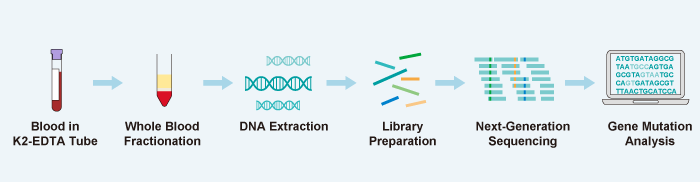
\includegraphics[width=\textwidth,height=0.7\textheight,keepaspectratio]{img/sequencing/seq1.png}
		\label{img:mot2}
		\caption{DNA sequencing in the analysis of mutations}
	\end{figure}
\end{frame}
%-------------------------------------------------------
%-------------------------------------------------------

%%%%%%%%%%%%%%%%%%%%%%%%%%%%%%%%%%%%%%%%%%%%%%%%%%%%%%%%%%%%%%%%%%%%%%%%%%%%%%%%%%%%%%%%%%%%%%%%%%%%%%%%%%%%%%%%
%%%%%%%%%%%%%%%%%%%%%%%%%%%%%%%%%%%%%%%%%%%%%%%%%%%%%%%%%%%%%%%%%%%%%%%%%%%%%%%%%%%%%%%%%%%%%%%%%%%%%%%%%%%%%%%%
%%%%%%%%%%%%%%%%%%%%%%%%%%%%%%%%%%%%%%%%%%%%%%%%%%%%%%%%%%%%%%%%%%%%%%%%%%%%%%%%%%%%%%%%%%%%%%%%%%%%%%%%%%%%%%%%
\section{Sanger DNA sequencing}
%%%%%%%%%%%%%%%%%%%%%%%%%%%%%%%%%%%%%%%%%%%%%%%%%%%%%%%%%%%%%%%%%%%%%%%%%%%%%%%%%%%%%%%%%%%%%%%%%%%%%%%%%%%%%%%%
%%%%%%%%%%%%%%%%%%%%%%%%%%%%%%%%%%%%%%%%%%%%%%%%%%%%%%%%%%%%%%%%%%%%%%%%%%%%%%%%%%%%%%%%%%%%%%%%%%%%%%%%%%%%%%%%
%%%%%%%%%%%%%%%%%%%%%%%%%%%%%%%%%%%%%%%%%%%%%%%%%%%%%%%%%%%%%%%%%%%%%%%%%%%%%%%%%%%%%%%%%%%%%%%%%%%%%%%%%%%%%%%%





%%%%%%%%%%%%%%%%%%%%%%%%%%%%%%%%%%%%%%%%%%%%%%%%%%%%%%%%%%%%%%%%%%%%%%%%%%%%%%%%%%%%%%%%%%%%%%%%%%%%%%%%%%%%%%%%
%%%%%%%%%%%%%%%%%%%%%%%%%%%%%%%%%%%%%%%%%%%%%%%%%%%%%%%%%%%%%%%%%%%%%%%%%%%%%%%%%%%%%%%%%%%%%%%%%%%%%%%%%%%%%%%%
%%%%%%%%%%%%%%%%%%%%%%%%%%%%%%%%%%%%%%%%%%%%%%%%%%%%%%%%%%%%%%%%%%%%%%%%%%%%%%%%%%%%%%%%%%%%%%%%%%%%%%%%%%%%%%%%
\subsection{Frederick Sanger}
%%%%%%%%%%%%%%%%%%%%%%%%%%%%%%%%%%%%%%%%%%%%%%%%%%%%%%%%%%%%%%%%%%%%%%%%%%%%%%%%%%%%%%%%%%%%%%%%%%%%%%%%%%%%%%%%
%%%%%%%%%%%%%%%%%%%%%%%%%%%%%%%%%%%%%%%%%%%%%%%%%%%%%%%%%%%%%%%%%%%%%%%%%%%%%%%%%%%%%%%%%%%%%%%%%%%%%%%%%%%%%%%%
%%%%%%%%%%%%%%%%%%%%%%%%%%%%%%%%%%%%%%%%%%%%%%%%%%%%%%%%%%%%%%%%%%%%%%%%%%%%%%%%%%%%%%%%%%%%%%%%%%%%%%%%%%%%%%%%

%-------------------------------------------------------
%-------------------------------------------------------
\begin{frame}{Sanger DNA sequencing}{Frederick Sanger}
	
		\begin{columns}
			\begin{column}{0.48\textwidth}
				\begin{block}{}
					Sanger (1975) proposed a method for determining sequences in DNA by primed synthesis with DNA polymerase \cite{sanger1977dna}. \\ 
					It is based on the principle of \textbf{Di deoxynucleotide}.
				\end{block} 
			\end{column}
			\begin{column}{0.48\textwidth}
				\begin{figure}[]
					\centering
					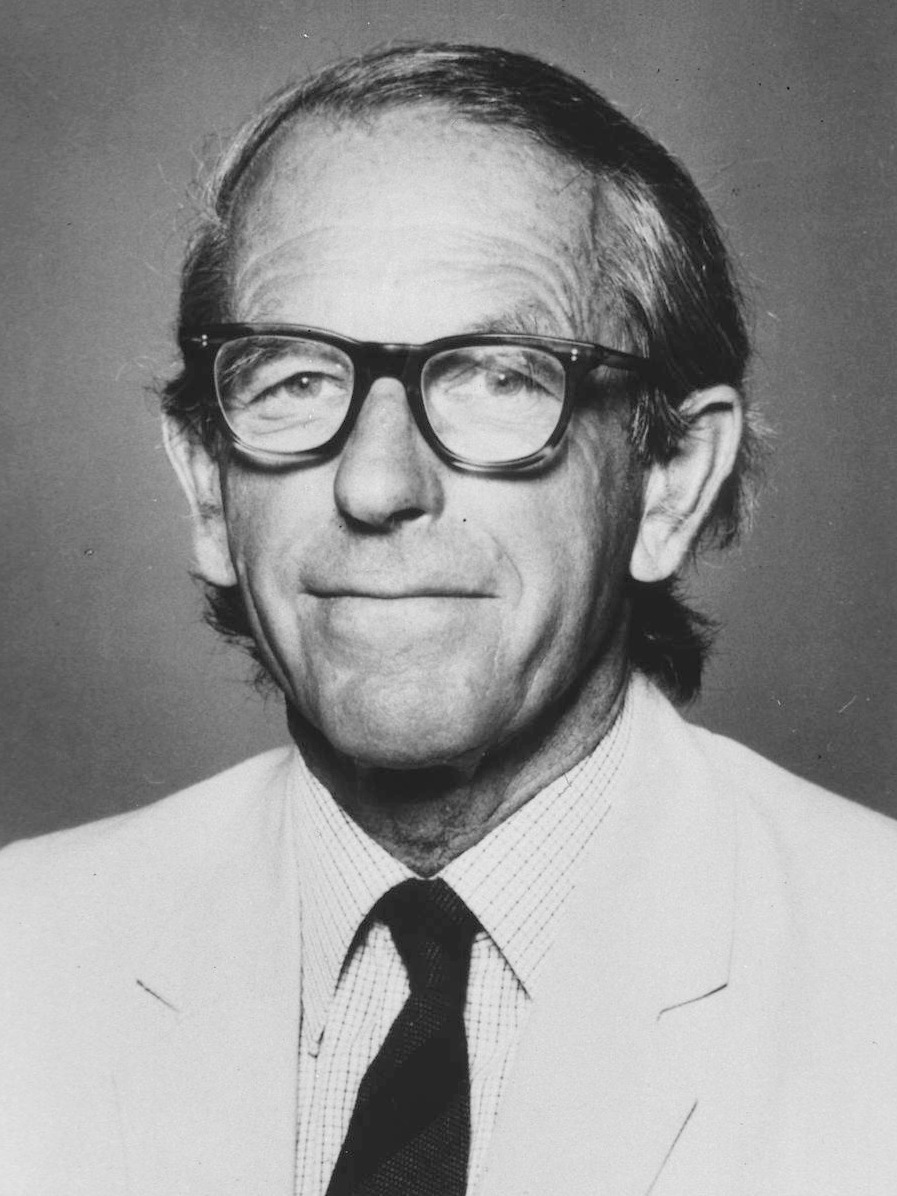
\includegraphics[width=\textwidth,height=0.5\textheight,keepaspectratio]{img/sequencing/sanger.jpg}
					\label{img:mot2}
					\caption{Frederick Sanger in 1977.}
				\end{figure}
			\end{column}
		\end{columns}	
\end{frame}
%-------------------------------------------------------
%-------------------------------------------------------

%%%%%%%%%%%%%%%%%%%%%%%%%%%%%%%%%%%%%%%%%%%%%%%%%%%%%%%%%%%%%%%%%%%%%%%%%%%%%%%%%%%%%%%%%%%%%%%%%%%%%%%%%%%%%%%%
%%%%%%%%%%%%%%%%%%%%%%%%%%%%%%%%%%%%%%%%%%%%%%%%%%%%%%%%%%%%%%%%%%%%%%%%%%%%%%%%%%%%%%%%%%%%%%%%%%%%%%%%%%%%%%%%
%%%%%%%%%%%%%%%%%%%%%%%%%%%%%%%%%%%%%%%%%%%%%%%%%%%%%%%%%%%%%%%%%%%%%%%%%%%%%%%%%%%%%%%%%%%%%%%%%%%%%%%%%%%%%%%%
\subsection{Di deoxynucleotide}
%%%%%%%%%%%%%%%%%%%%%%%%%%%%%%%%%%%%%%%%%%%%%%%%%%%%%%%%%%%%%%%%%%%%%%%%%%%%%%%%%%%%%%%%%%%%%%%%%%%%%%%%%%%%%%%%
%%%%%%%%%%%%%%%%%%%%%%%%%%%%%%%%%%%%%%%%%%%%%%%%%%%%%%%%%%%%%%%%%%%%%%%%%%%%%%%%%%%%%%%%%%%%%%%%%%%%%%%%%%%%%%%%
%%%%%%%%%%%%%%%%%%%%%%%%%%%%%%%%%%%%%%%%%%%%%%%%%%%%%%%%%%%%%%%%%%%%%%%%%%%%%%%%%%%%%%%%%%%%%%%%%%%%%%%%%%%%%%%%


%-------------------------------------------------------
%-------------------------------------------------------
\begin{frame}{Sanger method}{Deoxynucleotide}
	\begin{figure}[]
		\centering
		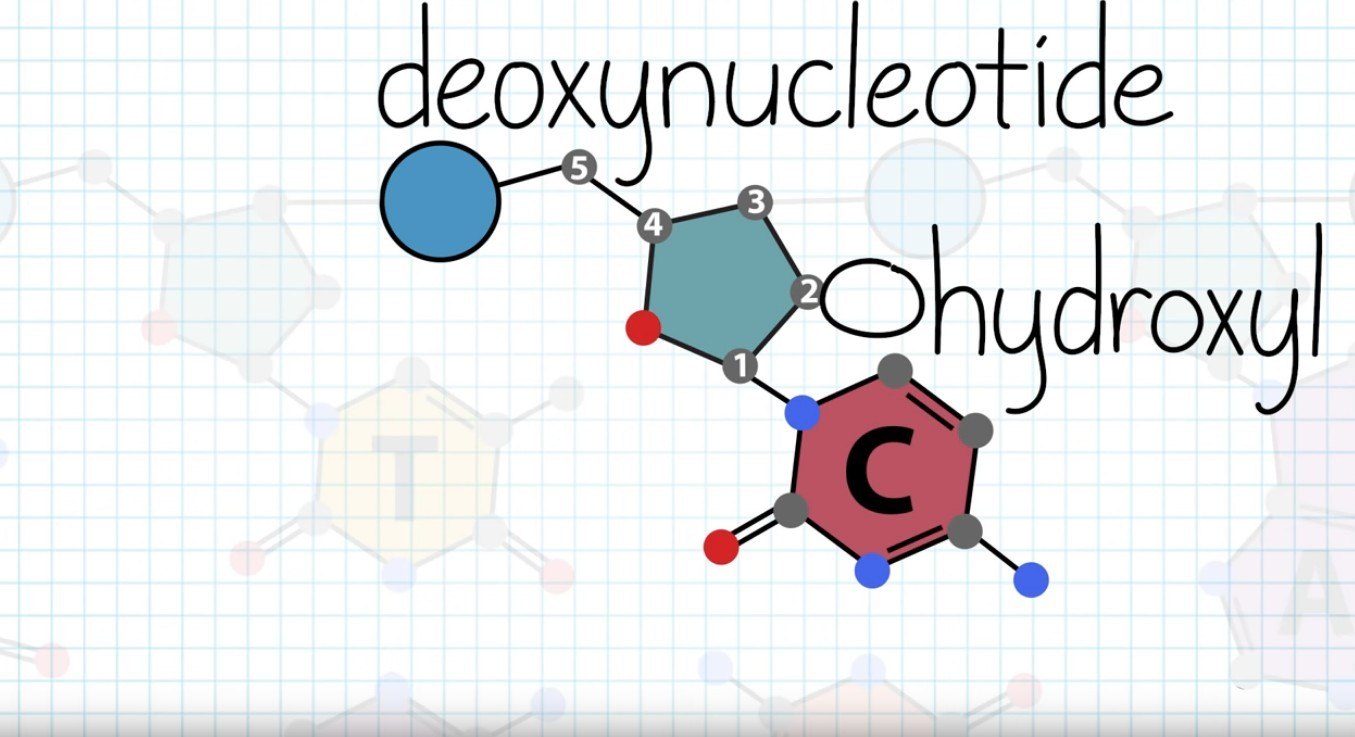
\includegraphics[width=\textwidth,height=0.7\textheight,keepaspectratio]{img/introduction/dna14.jpg}
		\label{img:mot2}
		\caption{The nucleotides are also called deoxynucleotides.}
	\end{figure}
\end{frame}
%-------------------------------------------------------
%-------------------------------------------------------

%-------------------------------------------------------
%-------------------------------------------------------
\begin{frame}{Sanger method}{dNTP}	
	\begin{block}{dNTP}
		Deoxynucleoside triphosphate \textbf{dNTPs} are standard natural substrates of all DNA polymerases.
	\end{block}
\end{frame}
%-------------------------------------------------------
%-------------------------------------------------------





%-------------------------------------------------------
%-------------------------------------------------------
\begin{frame}{Sanger method}{Deoxynucleotide}
	\begin{figure}[]
		\centering
		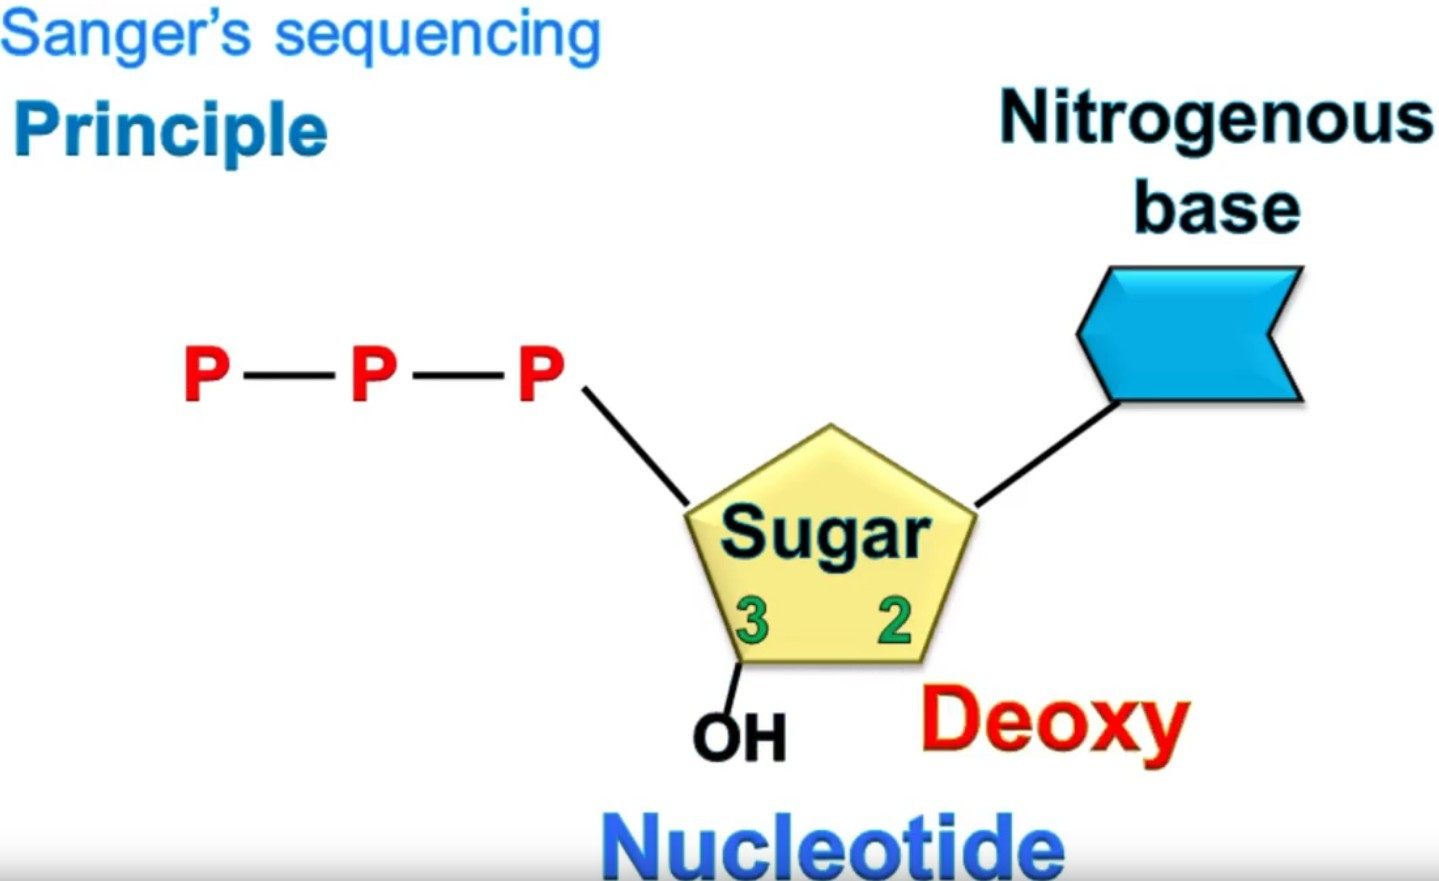
\includegraphics[width=\textwidth,height=0.6\textheight,keepaspectratio]{img/sequencing/seq2.jpg}
		\label{img:mot2}
		\caption{Deoxynucleotides doesn't have the hydroxyl group at the 2' carbon of sugar.}
	\end{figure}
\end{frame}
%-------------------------------------------------------
%-------------------------------------------------------

%-------------------------------------------------------
%-------------------------------------------------------
\begin{frame}{Sanger method}{Nucleotides and nucleosides}
	\begin{figure}[]
		\centering
		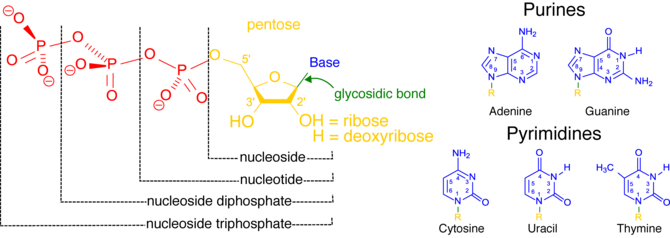
\includegraphics[width=\textwidth,height=0.6\textheight,keepaspectratio]{img/sequencing/seq3.png}
		\label{img:mot2}
		\caption{The difference of nucleotides and nucleosides.}
	\end{figure}
\end{frame}
%-------------------------------------------------------
%-------------------------------------------------------

%-------------------------------------------------------
%-------------------------------------------------------
\begin{frame}{Sanger method}{Deoxynucleotide}
	\begin{figure}[]
		\centering
		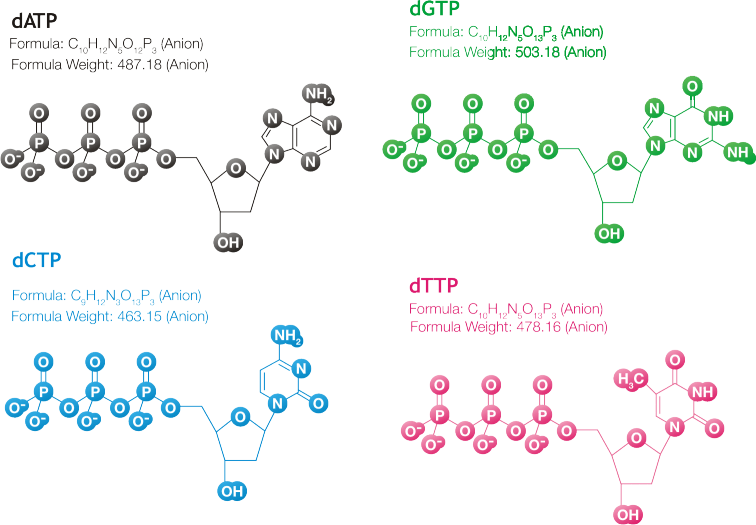
\includegraphics[width=\textwidth,height=0.7\textheight,keepaspectratio]{img/sequencing/seq10.png}
		\label{img:mot2}
		\caption{Deoxynucleotides: dATP, dTTP, dCTP and dGTP.}
	\end{figure}
\end{frame}
%-------------------------------------------------------
%-------------------------------------------------------


%-------------------------------------------------------
%-------------------------------------------------------
\begin{frame}{Sanger method}{DNA replication - Di Deoxynucletide principle}
	\begin{figure}[]
		\centering
		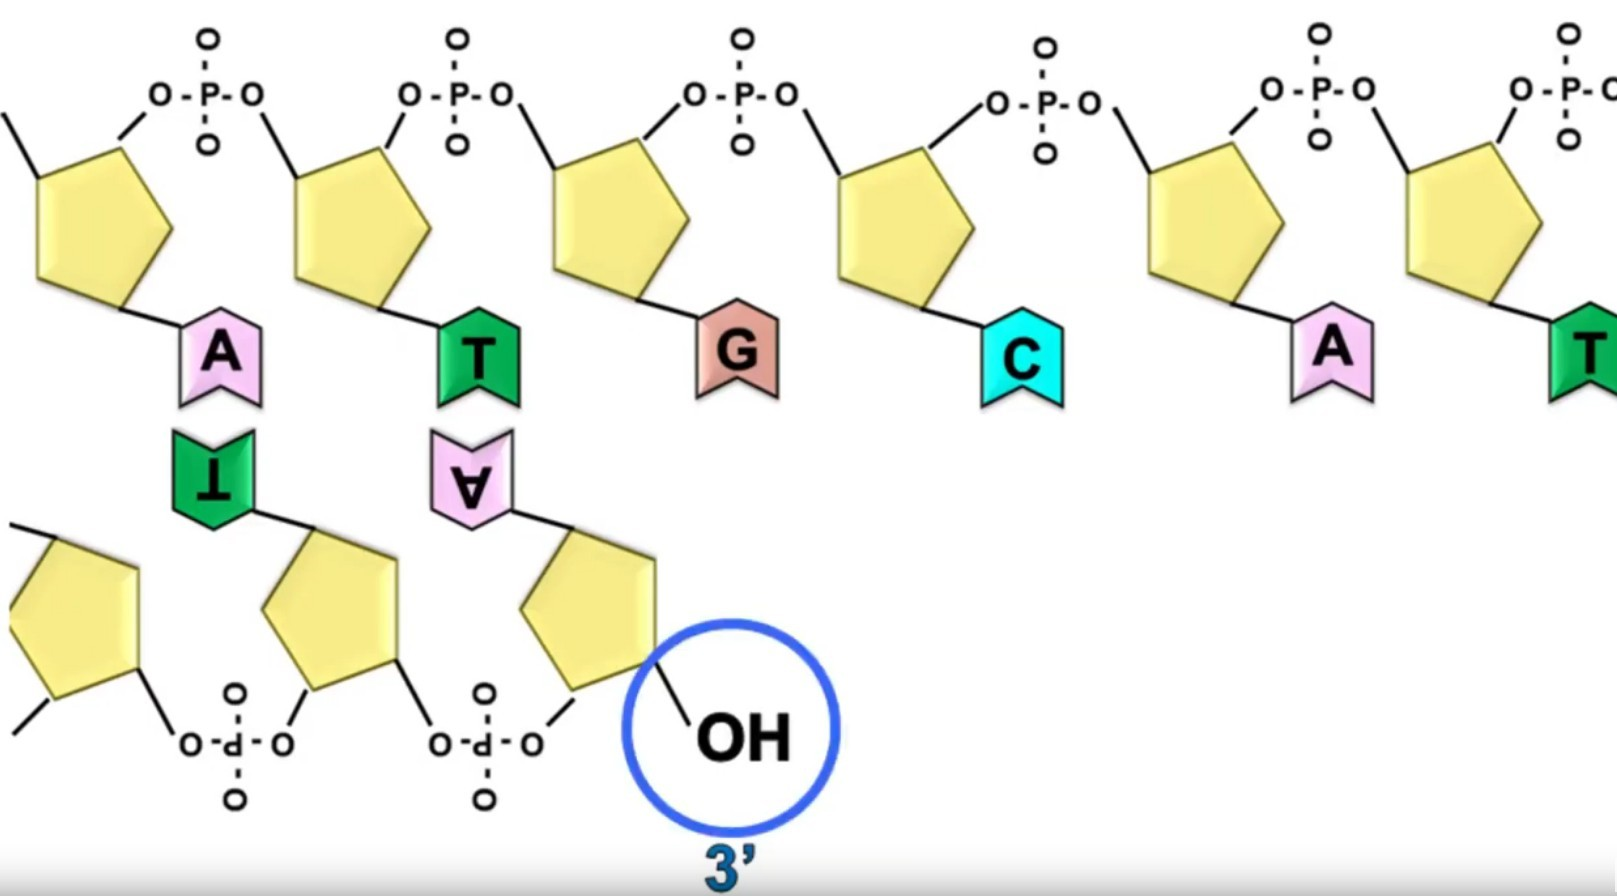
\includegraphics[width=\textwidth,height=0.6\textheight,keepaspectratio]{img/sequencing/seq4.jpg}
		\label{img:mot2}
		\caption{dNTPs are attached to the 3' carbon of sugar.}
	\end{figure}
\end{frame}
%-------------------------------------------------------
%-------------------------------------------------------

%-------------------------------------------------------
%-------------------------------------------------------
\begin{frame}{Sanger method}{DNA replication - Di Deoxynucletide principle}
	\begin{figure}[]
		\centering
		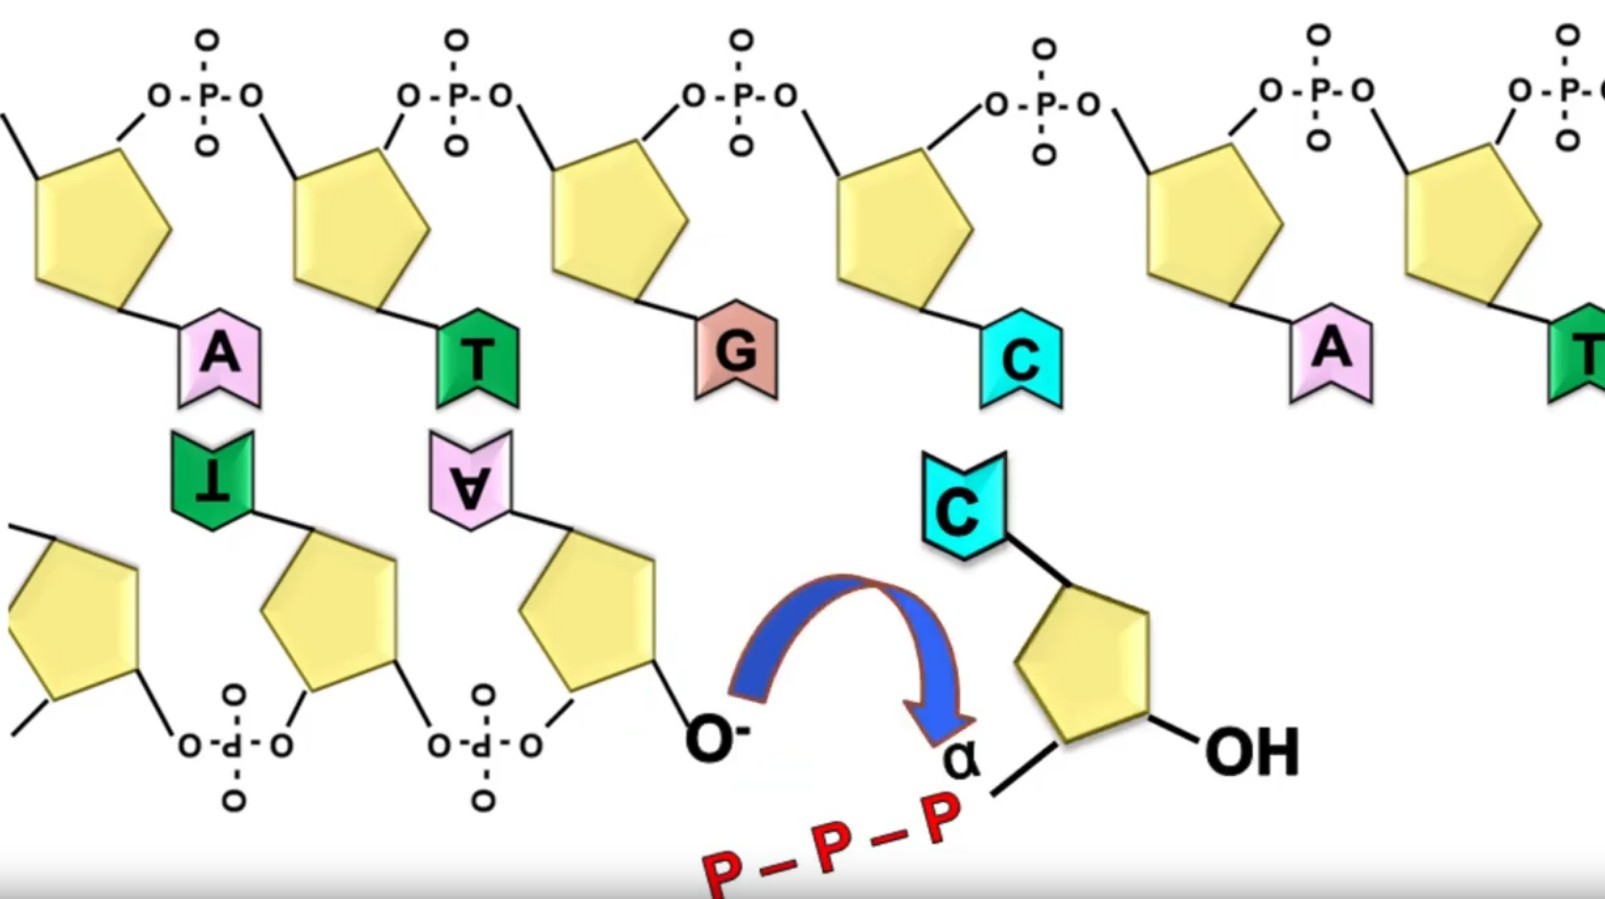
\includegraphics[width=\textwidth,height=0.6\textheight,keepaspectratio]{img/sequencing/seq5.jpg}
		\label{img:mot2}
		\caption{dNTPs are attached to the 3' carbon of sugar.}
	\end{figure}
\end{frame}
%-------------------------------------------------------
%-------------------------------------------------------

%-------------------------------------------------------
%-------------------------------------------------------
\begin{frame}{Sanger method}{DNA replication - Di Deoxynucletide principle}
	\begin{figure}[]
		\centering
		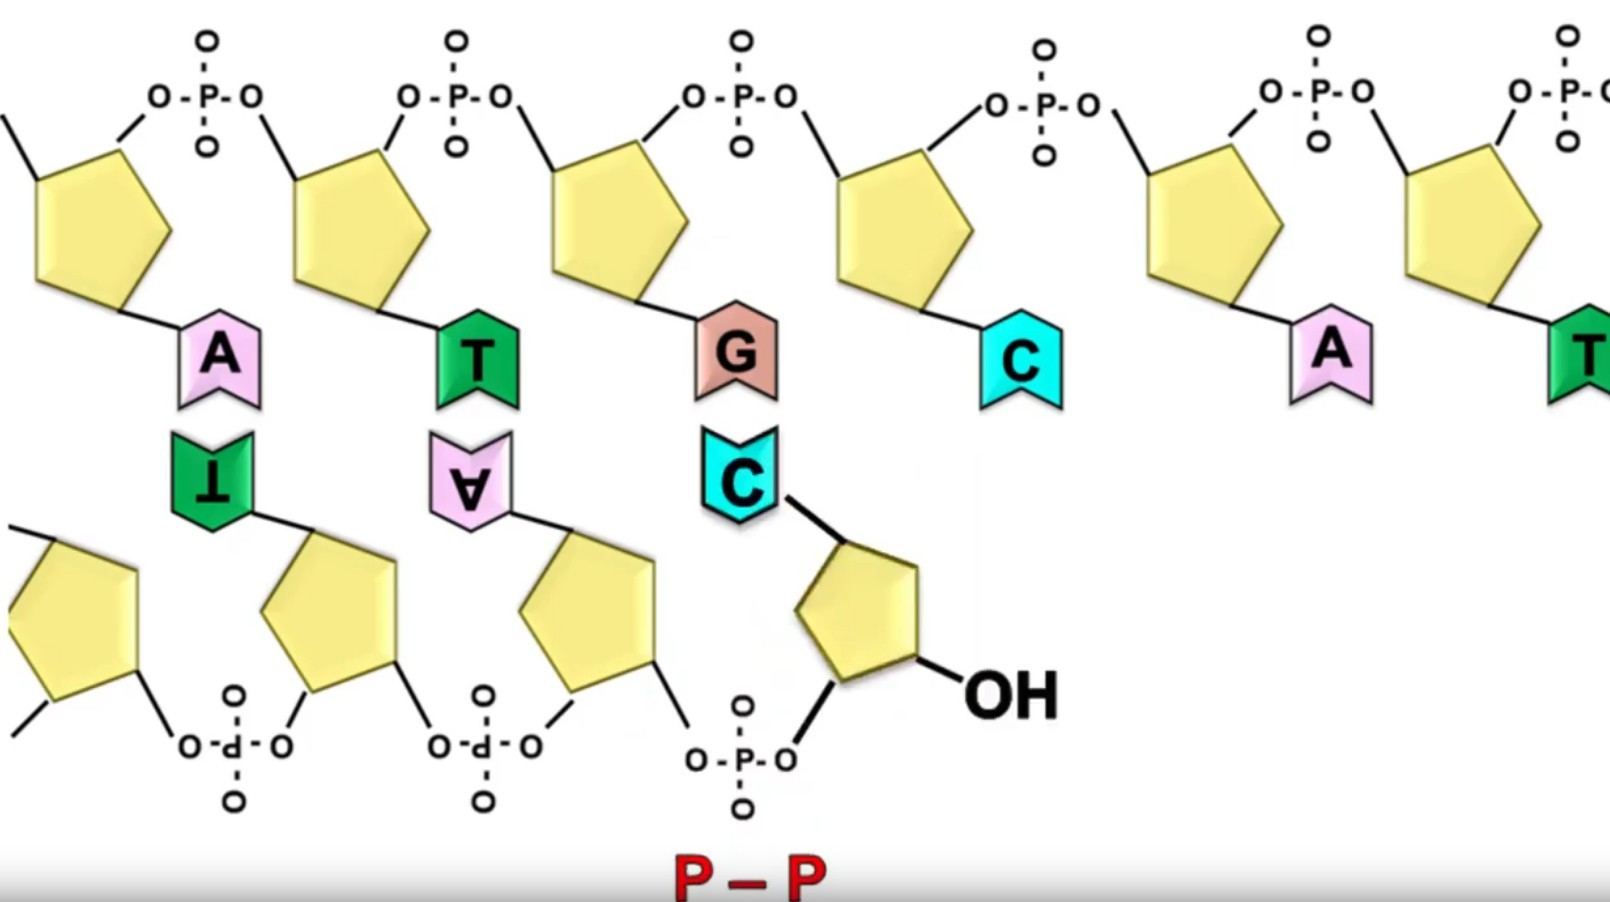
\includegraphics[width=\textwidth,height=0.6\textheight,keepaspectratio]{img/sequencing/seq6.jpg}
		\label{img:mot2}
		\caption{dNTPs are attached to the 3' carbon of sugar.}
	\end{figure}
\end{frame}
%-------------------------------------------------------
%-------------------------------------------------------


%-------------------------------------------------------
%-------------------------------------------------------
\begin{frame}{Sanger method}{DNA replication - Di Deoxynucletide principle}
	\begin{figure}[]
		\centering
		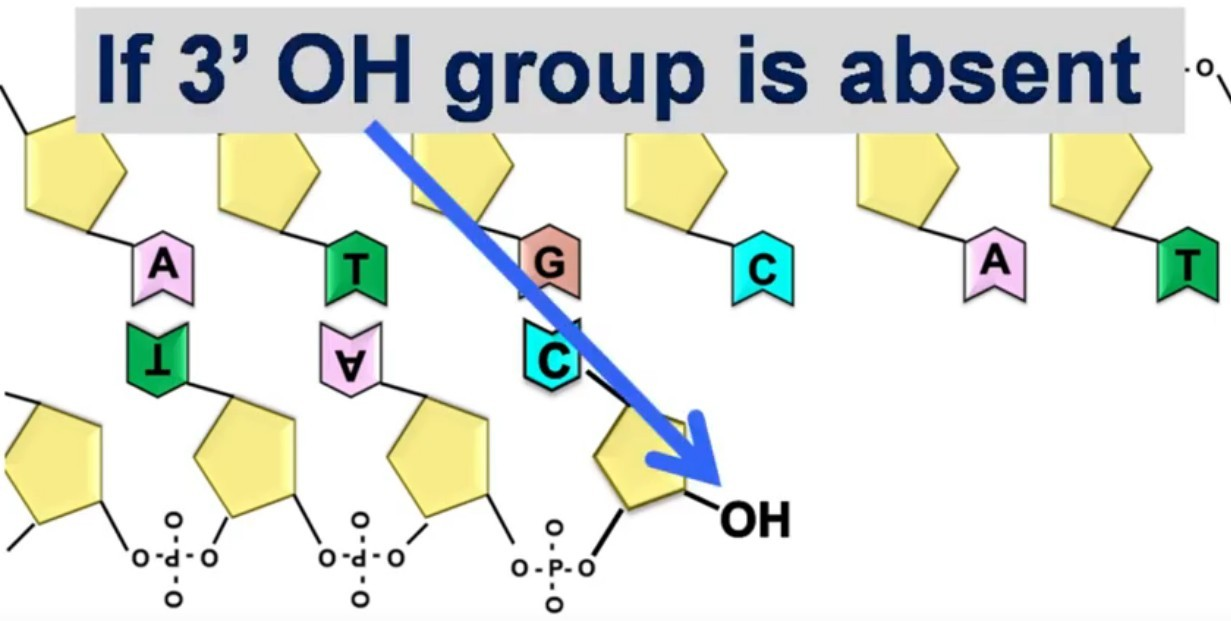
\includegraphics[width=\textwidth,height=0.6\textheight,keepaspectratio]{img/sequencing/seq7.jpg}
		\label{img:mot2}
		\caption{If 3' OH group is absent, the reaction stop.}
	\end{figure}
\end{frame}
%-------------------------------------------------------
%-------------------------------------------------------


%-------------------------------------------------------
%-------------------------------------------------------
\begin{frame}{Sanger method}{DNA replication - Di Deoxynucletide principle}
	\begin{figure}[]
		\centering
		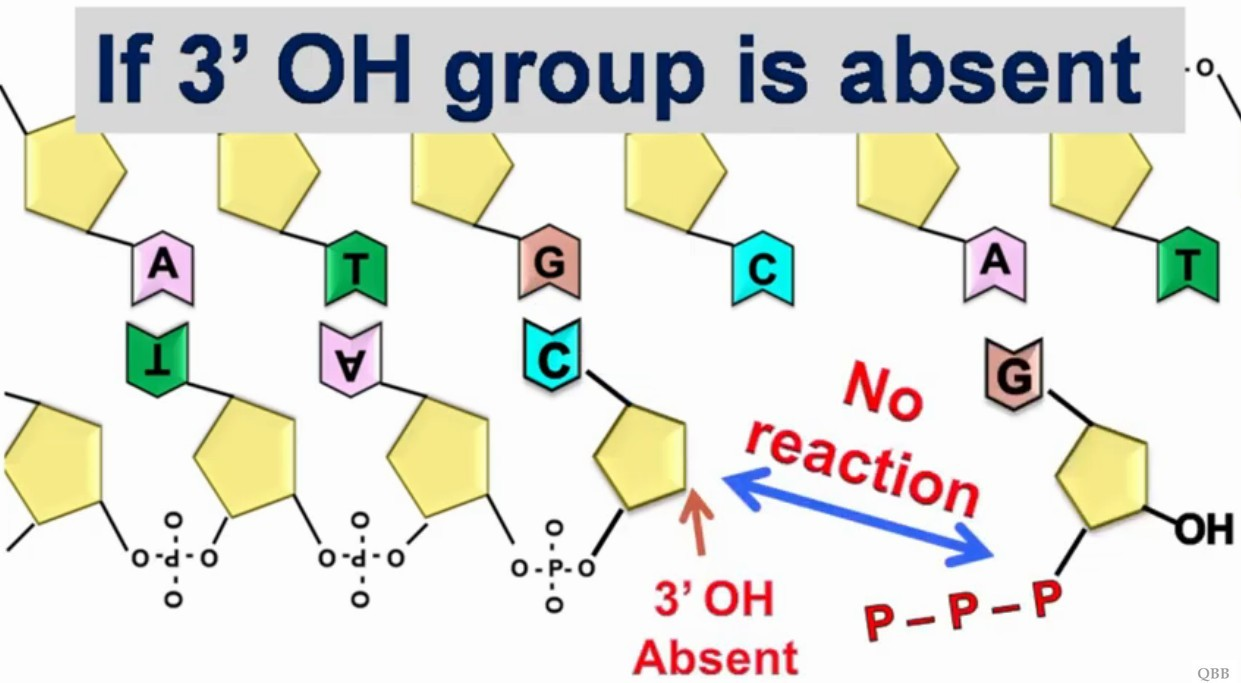
\includegraphics[width=\textwidth,height=0.6\textheight,keepaspectratio]{img/sequencing/seq8.jpg}
		\label{img:mot2}
		\caption{If 3' OH group is absent, the reaction stop.}
	\end{figure}
\end{frame}
%-------------------------------------------------------
%-------------------------------------------------------

%-------------------------------------------------------
%-------------------------------------------------------
\begin{frame}{Sanger method}{Deoxynucleotide}
	\begin{figure}[]
		\centering
		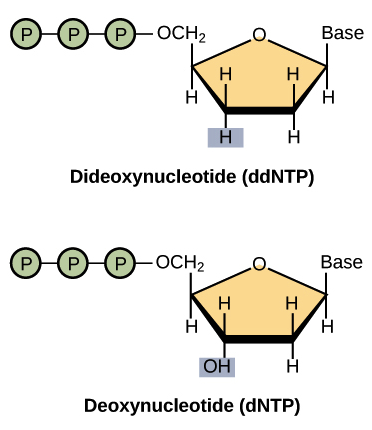
\includegraphics[width=\textwidth,height=0.7\textheight,keepaspectratio]{img/sequencing/seq9.png}
		\label{img:mot2}
		\caption{Deoxynucleotide and Di Deoxynucletide.}
	\end{figure}
\end{frame}
%-------------------------------------------------------
%-------------------------------------------------------

%%%%%%%%%%%%%%%%%%%%%%%%%%%%%%%%%%%%%%%%%%%%%%%%%%%%%%%%%%%%%%%%%%%%%%%%%%%%%%%%%%%%%%%%%%%%%%%%%%%%%%%%%%%%%%%%
%%%%%%%%%%%%%%%%%%%%%%%%%%%%%%%%%%%%%%%%%%%%%%%%%%%%%%%%%%%%%%%%%%%%%%%%%%%%%%%%%%%%%%%%%%%%%%%%%%%%%%%%%%%%%%%%
%%%%%%%%%%%%%%%%%%%%%%%%%%%%%%%%%%%%%%%%%%%%%%%%%%%%%%%%%%%%%%%%%%%%%%%%%%%%%%%%%%%%%%%%%%%%%%%%%%%%%%%%%%%%%%%%
\subsection{Sanger Method - Gel Electrophoresis}
%%%%%%%%%%%%%%%%%%%%%%%%%%%%%%%%%%%%%%%%%%%%%%%%%%%%%%%%%%%%%%%%%%%%%%%%%%%%%%%%%%%%%%%%%%%%%%%%%%%%%%%%%%%%%%%%
%%%%%%%%%%%%%%%%%%%%%%%%%%%%%%%%%%%%%%%%%%%%%%%%%%%%%%%%%%%%%%%%%%%%%%%%%%%%%%%%%%%%%%%%%%%%%%%%%%%%%%%%%%%%%%%%
%%%%%%%%%%%%%%%%%%%%%%%%%%%%%%%%%%%%%%%%%%%%%%%%%%%%%%%%%%%%%%%%%%%%%%%%%%%%%%%%%%%%%%%%%%%%%%%%%%%%%%%%%%%%%%%%

%-------------------------------------------------------
%-------------------------------------------------------
\begin{frame}{Sanger method}{Double helix DNA}
	\begin{figure}[]
		\centering
		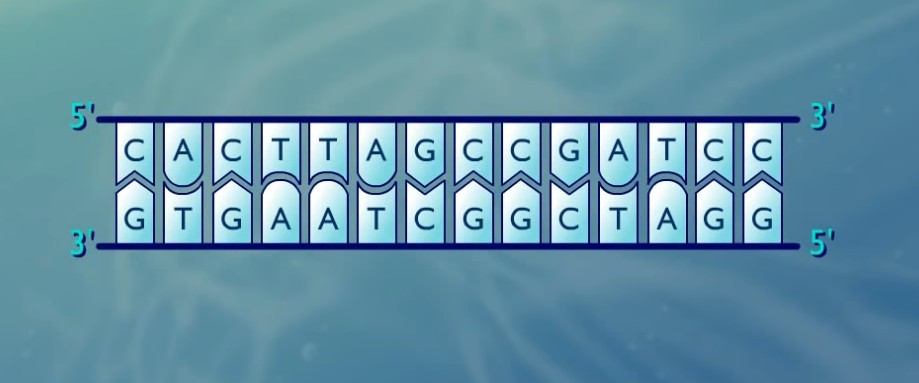
\includegraphics[width=\textwidth,height=0.7\textheight,keepaspectratio]{img/sequencing/seq11.jpg}
		\label{img:mot2}
		\caption{The Sanger method start from a double helix DNA.}
	\end{figure}
\end{frame}
%-------------------------------------------------------
%-------------------------------------------------------

%-------------------------------------------------------
%-------------------------------------------------------
\begin{frame}{Sanger method}{Single strand DNA}
	\begin{figure}[]
		\centering
		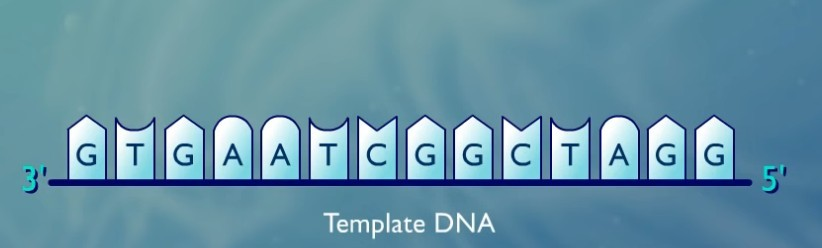
\includegraphics[width=\textwidth,height=0.7\textheight,keepaspectratio]{img/sequencing/seq12.jpg}
		\label{img:mot2}
		\caption{The double helix DNA is separated with high temperatures.}
	\end{figure}
\end{frame}
%-------------------------------------------------------
%-------------------------------------------------------


%-------------------------------------------------------
%-------------------------------------------------------
\begin{frame}{Sanger method}{Primer - dNTPs - DNA Polymerase}
	\begin{figure}[]
		\centering
		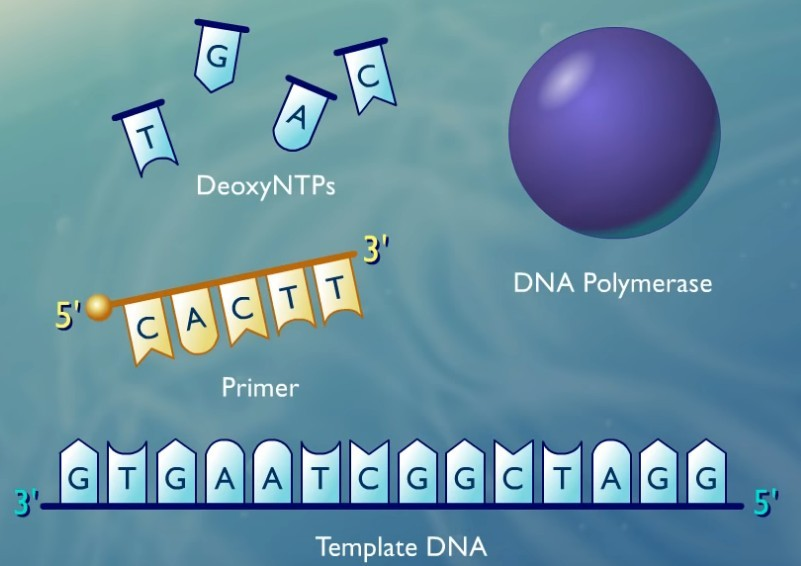
\includegraphics[width=\textwidth,height=0.7\textheight,keepaspectratio]{img/sequencing/seq13.jpg}
		\label{img:mot2}
		\caption{Three components are prepared in vitro. dNTPs, DNA Polymerase and a Primer.}
	\end{figure}
\end{frame}
%-------------------------------------------------------
%-------------------------------------------------------






%-------------------------------------------------------
%-------------------------------------------------------
\begin{frame}{Sanger method}{Primer - dNTPs - DNA Polymerase}
	\begin{figure}[]
		\centering
		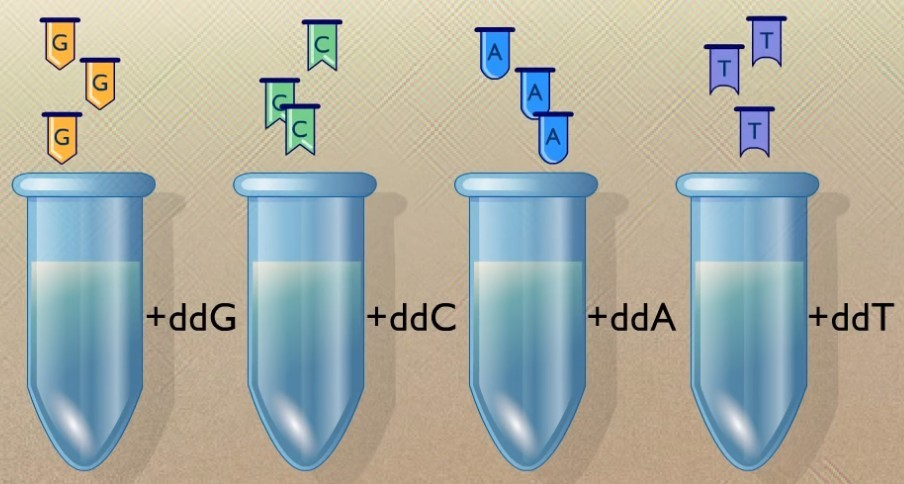
\includegraphics[width=\textwidth,height=0.7\textheight,keepaspectratio]{img/sequencing/seq14.jpg}
		\label{img:mot2}
		\caption{Four tubes are used. Each tube contains: DNA template, primer, dNTPs, DNA polymerase and one type of ddNTP (ATP or TTP or CTP or GTP).}
	\end{figure}
\end{frame}
%-------------------------------------------------------
%-------------------------------------------------------



%-------------------------------------------------------
%-------------------------------------------------------
\begin{frame}{Sanger method}{Radioactive phosphorus labeled}
	\begin{figure}[]
		\centering
		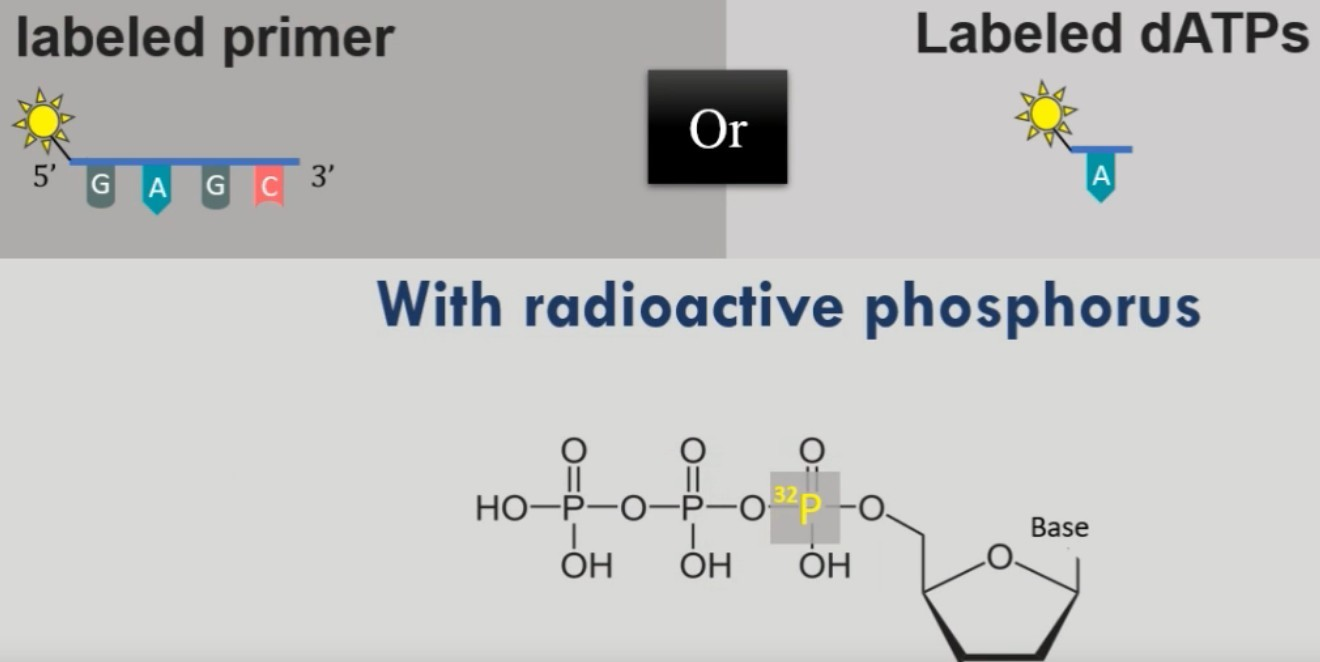
\includegraphics[width=\textwidth,height=0.7\textheight,keepaspectratio]{img/sequencing/seq23.jpg}
		\label{img:mot2}
		\caption{Before starting the reaction, the primer or one of dNTPs are labeled.}
	\end{figure}
\end{frame}
%-------------------------------------------------------
%-------------------------------------------------------




%-------------------------------------------------------
%-------------------------------------------------------
\begin{frame}{Sanger method}{DNA replication in each tube}
	\begin{figure}[]
		\centering
		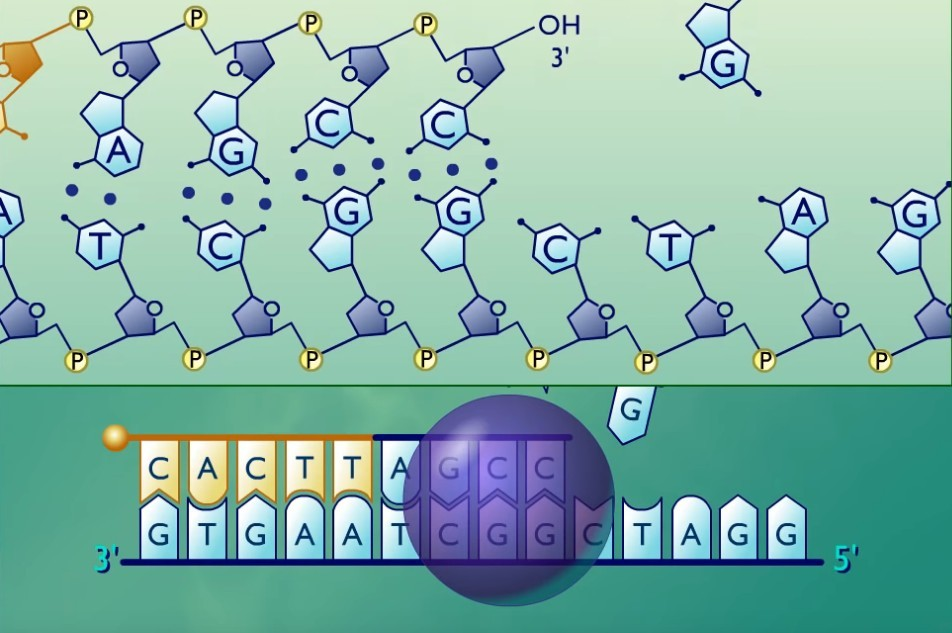
\includegraphics[width=\textwidth,height=0.7\textheight,keepaspectratio]{img/sequencing/seq15.jpg}
		\label{img:mot2}
		\caption{DNA replication occurs in each tube. The tubes contains the dNTPs.}
	\end{figure}
\end{frame}
%-------------------------------------------------------
%-------------------------------------------------------

%-------------------------------------------------------
%-------------------------------------------------------
\begin{frame}{Sanger method}{DNA replication stop when ddNTP arrives}
	\begin{figure}[]
		\centering
		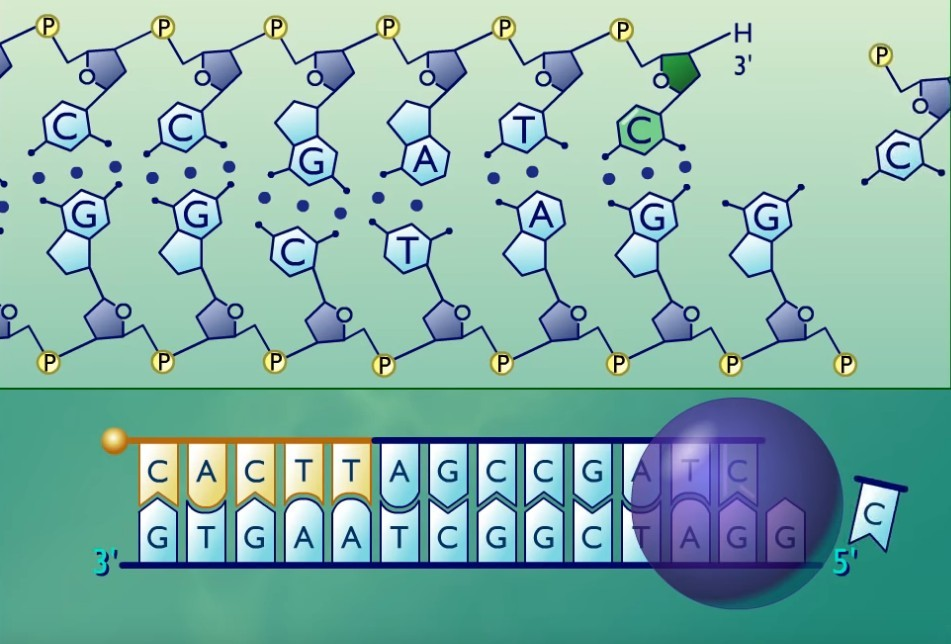
\includegraphics[width=\textwidth,height=0.7\textheight,keepaspectratio]{img/sequencing/seq16.jpg}
		\label{img:mot2}
		\caption{DNA replication stop when a ddNTP arrives.}
	\end{figure}
\end{frame}
%-------------------------------------------------------
%-------------------------------------------------------


%-------------------------------------------------------
%-------------------------------------------------------
\begin{frame}{Sanger method}{DNA replication starts again}
	\begin{figure}[]
		\centering
		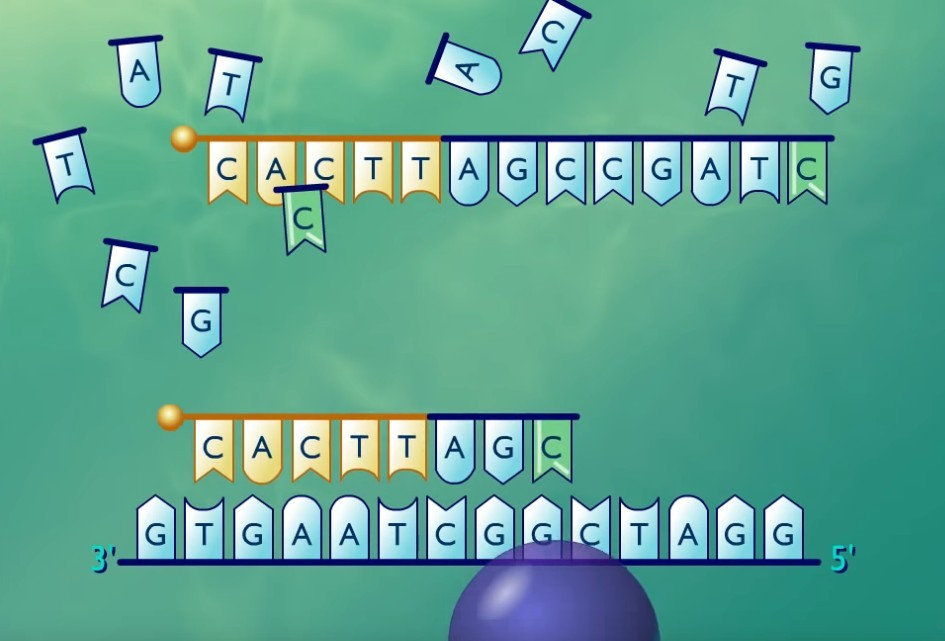
\includegraphics[width=\textwidth,height=0.7\textheight,keepaspectratio]{img/sequencing/seq17.jpg}
		\label{img:mot2}
		\caption{DNA replication starts again and different fragments length are obtained.}
	\end{figure}
\end{frame}
%-------------------------------------------------------
%-------------------------------------------------------


%-------------------------------------------------------
%-------------------------------------------------------
\begin{frame}{Sanger method}{DNA replication starts again}
	\begin{figure}[]
		\centering
		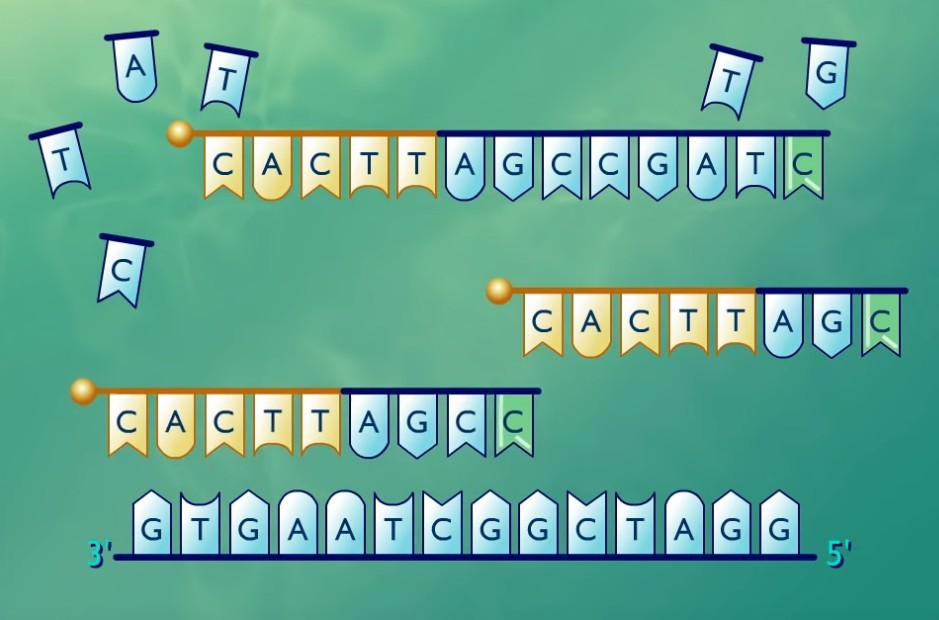
\includegraphics[width=\textwidth,height=0.7\textheight,keepaspectratio]{img/sequencing/seq18.jpg}
		\label{img:mot2}
		\caption{DNA replication starts again and different fragments are obtained.}
	\end{figure}
\end{frame}
%-------------------------------------------------------
%-------------------------------------------------------


%-------------------------------------------------------
%-------------------------------------------------------
\begin{frame}{Sanger method}{Each tube have fragments of DNA}
	\begin{figure}[]
		\centering
		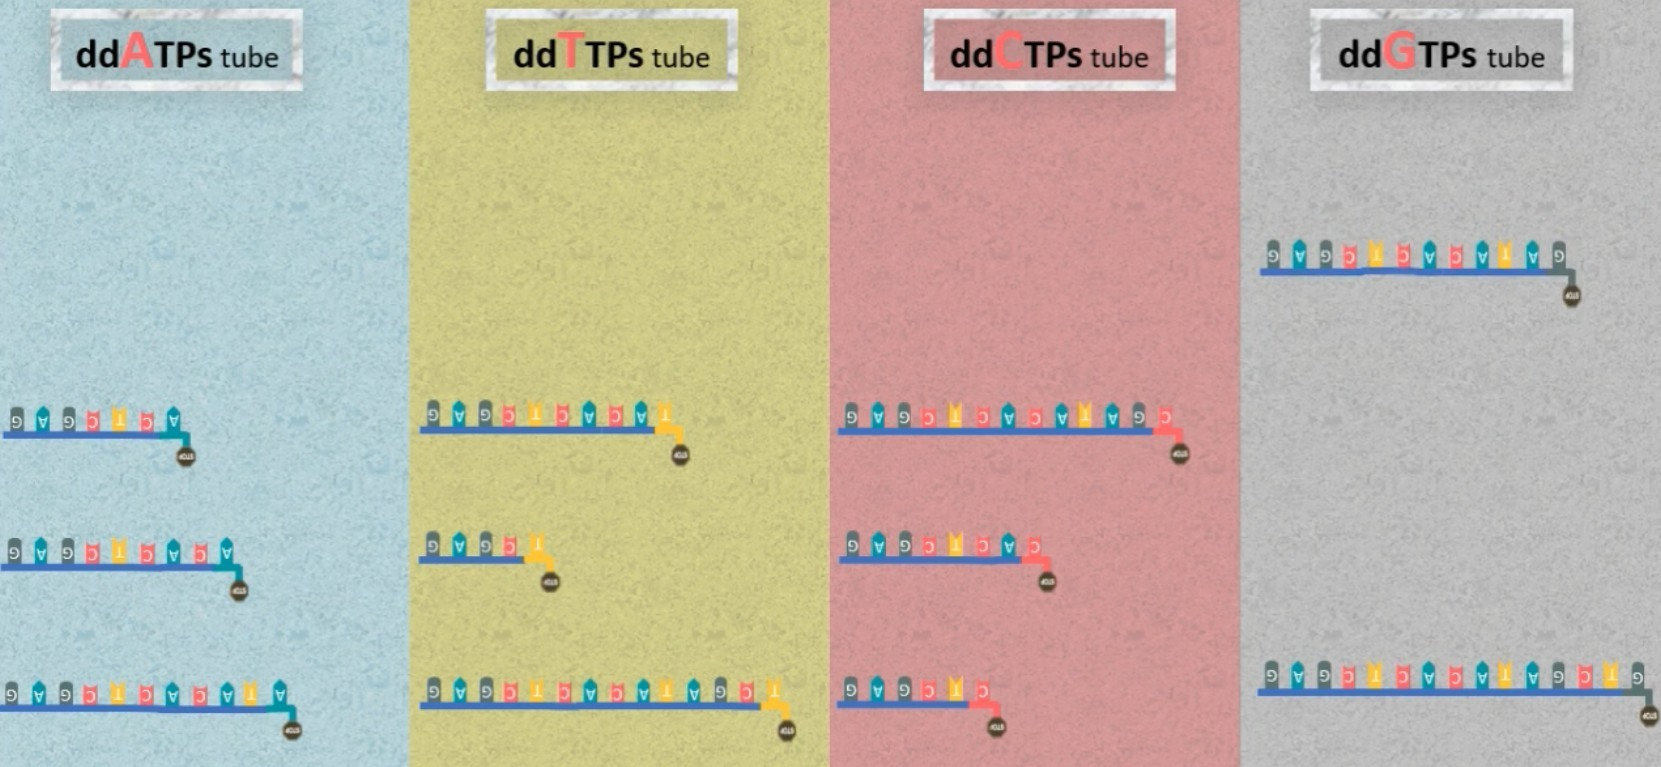
\includegraphics[width=\textwidth,height=0.7\textheight,keepaspectratio]{img/sequencing/seq24.jpg}
		\label{img:mot2}
		\caption{On each tube, there are DNA fragments, each one with different length.}
	\end{figure}
\end{frame}
%-------------------------------------------------------
%-------------------------------------------------------

%-------------------------------------------------------
%-------------------------------------------------------
\begin{frame}{Sanger method}{Gel electrophoresis}
	\begin{figure}[]
		\centering
		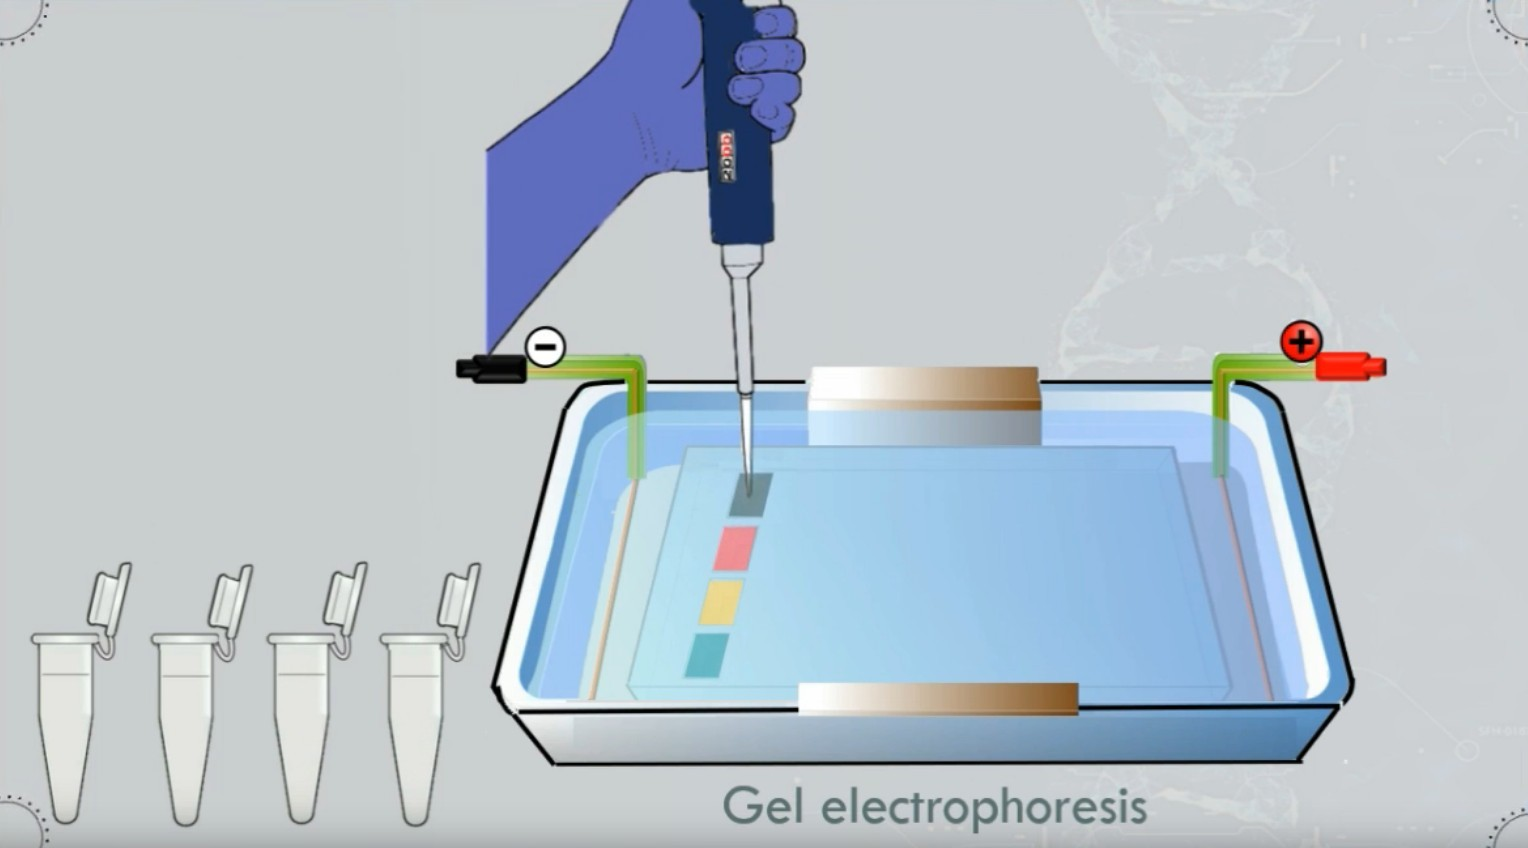
\includegraphics[width=\textwidth,height=0.7\textheight,keepaspectratio]{img/sequencing/seq25.jpg}
		\label{img:mot2}
		\caption{Gel electrophoresis. The negative charge of its phosphate backbone moves the DNA towards the positively charge anode.}
	\end{figure}
\end{frame}
%-------------------------------------------------------
%-------------------------------------------------------

%-------------------------------------------------------
%-------------------------------------------------------
\begin{frame}{Sanger method}{Gel electrophoresis}
	\begin{figure}[]
		\centering
		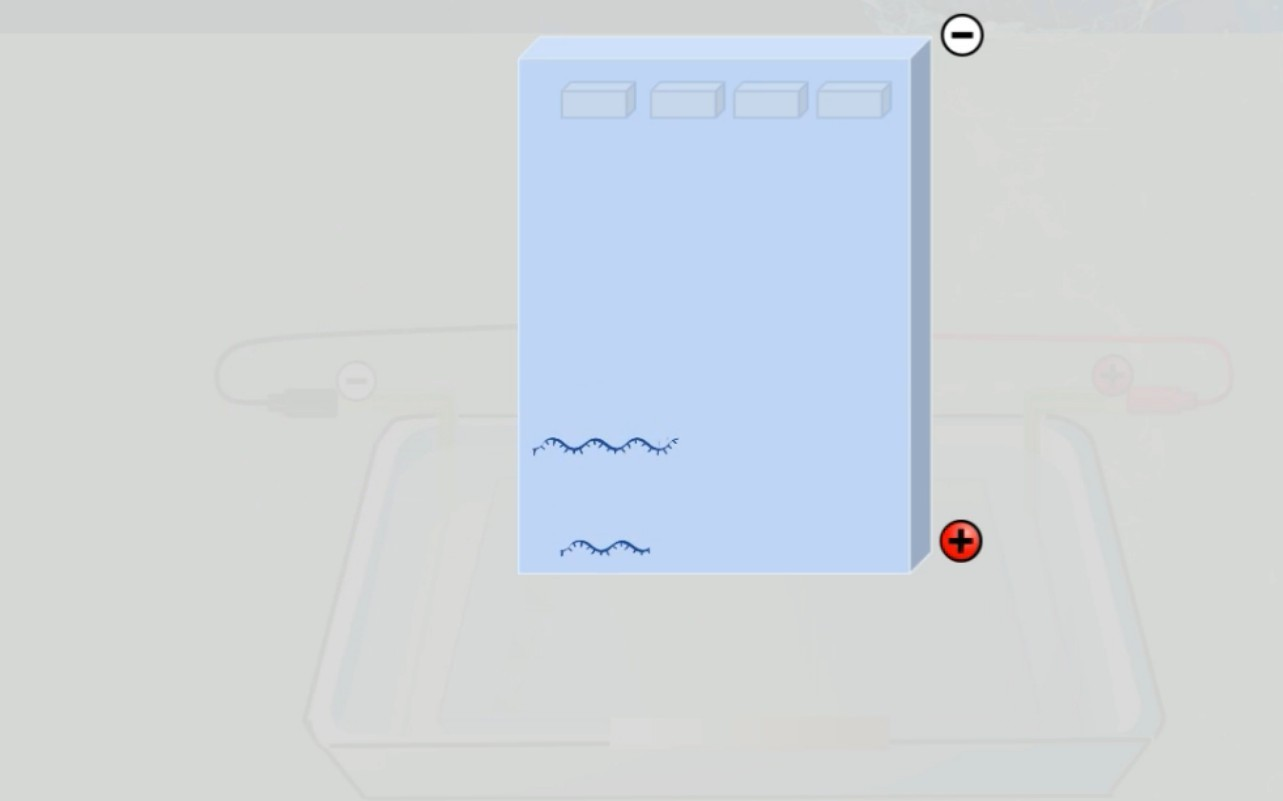
\includegraphics[width=\textwidth,height=0.7\textheight,keepaspectratio]{img/sequencing/seq26.jpg}
		\label{img:mot2}
		\caption{Shorter DNA molecules can travel farther than longer counterparts.}
	\end{figure}
\end{frame}
%-------------------------------------------------------
%-------------------------------------------------------

%-------------------------------------------------------
%-------------------------------------------------------
\begin{frame}{Sanger method}{Gel electrophoresis}
	\begin{figure}[]
		\centering
		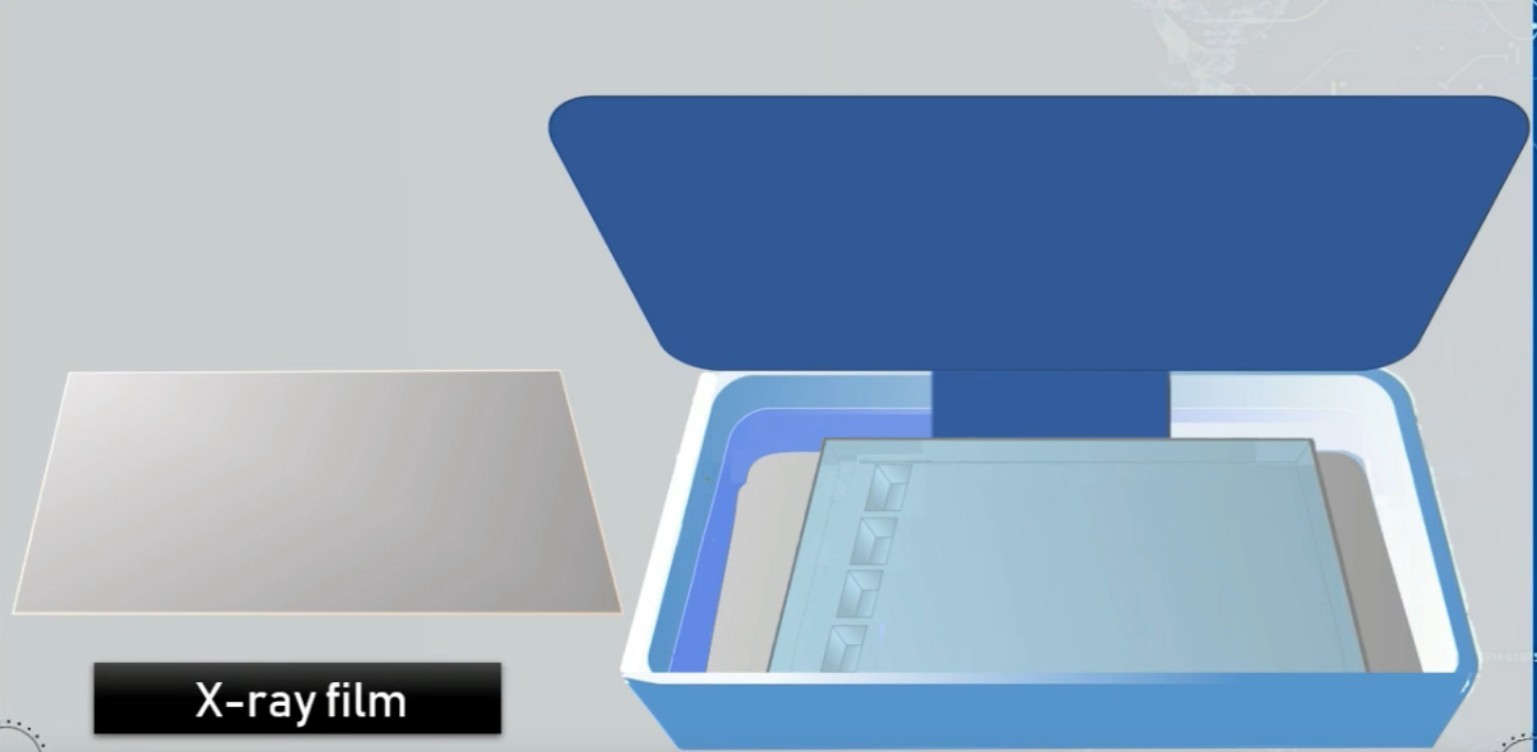
\includegraphics[width=\textwidth,height=0.7\textheight,keepaspectratio]{img/sequencing/seq28.jpg}
		\label{img:mot2}
		\caption{Tha DNA bands are visualized by autoradiography using the X-ray film.}
	\end{figure}
\end{frame}
%-------------------------------------------------------
%-------------------------------------------------------


%-------------------------------------------------------
%-------------------------------------------------------
\begin{frame}{Sanger method}{Gel electrophoresis}
	\begin{figure}[]
		\centering
		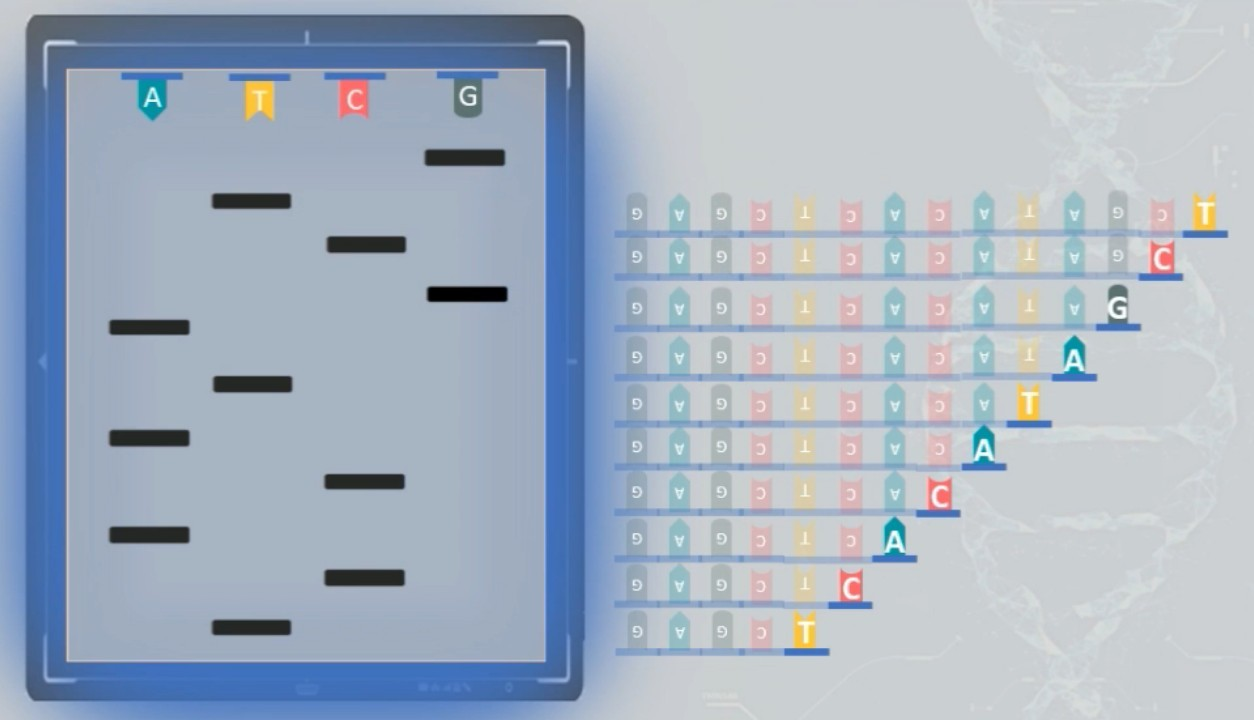
\includegraphics[width=\textwidth,height=0.7\textheight,keepaspectratio]{img/sequencing/seq27.jpg}
		\label{img:mot2}
		\caption{Tha DNA bands are visualized by autoradiography using the X-ray film.}
	\end{figure}
\end{frame}
%-------------------------------------------------------
%-------------------------------------------------------

%-------------------------------------------------------
%-------------------------------------------------------%
%\begin{frame}{Sanger method}{Each tube have fragments of DNA}
%	\begin{figure}[]
%		\centering
%		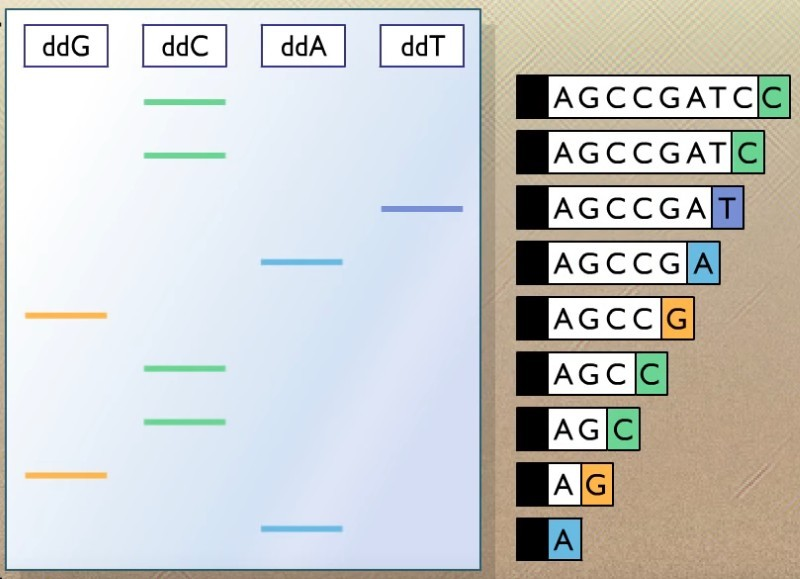
\includegraphics[width=\textwidth,height=0.5\textheight,keepaspectratio]{img/sequencing/seq19.jpg}
%		\label{img:mot2}
%		\caption{On each tube, there are DNA fragments, each one with different length.}
%	\end{figure}
%\end{frame}
%-------------------------------------------------------
%-------------------------------------------------------

%-------------------------------------------------------
%-------------------------------------------------------
\begin{frame}{Sanger method}{Gel Electrophoresis Animation}
	\begin{block}{}
		\href{https://www.youtube.com/watch?v=YeHtjO7vlyg&t=20s}{Gel Electrophoresis Animation.}
		
	\end{block}
\end{frame}
%-------------------------------------------------------
%-------------------------------------------------------




%%%%%%%%%%%%%%%%%%%%%%%%%%%%%%%%%%%%%%%%%%%%%%%%%%%%%%%%%%%%%%%%%%%%%%%%%%%%%%%%%%%%%%%%%%%%%%%%%%%%%%%%%%%%%%%%
%%%%%%%%%%%%%%%%%%%%%%%%%%%%%%%%%%%%%%%%%%%%%%%%%%%%%%%%%%%%%%%%%%%%%%%%%%%%%%%%%%%%%%%%%%%%%%%%%%%%%%%%%%%%%%%%
%%%%%%%%%%%%%%%%%%%%%%%%%%%%%%%%%%%%%%%%%%%%%%%%%%%%%%%%%%%%%%%%%%%%%%%%%%%%%%%%%%%%%%%%%%%%%%%%%%%%%%%%%%%%%%%%
\subsection{Sanger Method - Capilar Electrophoresis}
%%%%%%%%%%%%%%%%%%%%%%%%%%%%%%%%%%%%%%%%%%%%%%%%%%%%%%%%%%%%%%%%%%%%%%%%%%%%%%%%%%%%%%%%%%%%%%%%%%%%%%%%%%%%%%%%
%%%%%%%%%%%%%%%%%%%%%%%%%%%%%%%%%%%%%%%%%%%%%%%%%%%%%%%%%%%%%%%%%%%%%%%%%%%%%%%%%%%%%%%%%%%%%%%%%%%%%%%%%%%%%%%%
%%%%%%%%%%%%%%%%%%%%%%%%%%%%%%%%%%%%%%%%%%%%%%%%%%%%%%%%%%%%%%%%%%%%%%%%%%%%%%%%%%%%%%%%%%%%%%%%%%%%%%%%%%%%%%%%



%-------------------------------------------------------
%-------------------------------------------------------
\begin{frame}{Sanger method}{Capilar Electrophoresis}
	\begin{figure}[]
		\centering
		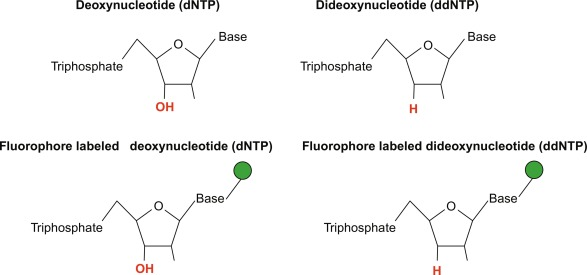
\includegraphics[width=\textwidth,height=0.7\textheight,keepaspectratio]{img/sequencing/seq21.jpg}
		\label{img:mot2}
		\caption{The ddNTPs are fluorophore labeled.}
	\end{figure}
\end{frame}
%-------------------------------------------------------
%-------------------------------------------------------

%-------------------------------------------------------
%-------------------------------------------------------
\begin{frame}{Sanger method}{Capilar Electrophoresis}
	\begin{figure}[]
		\centering
		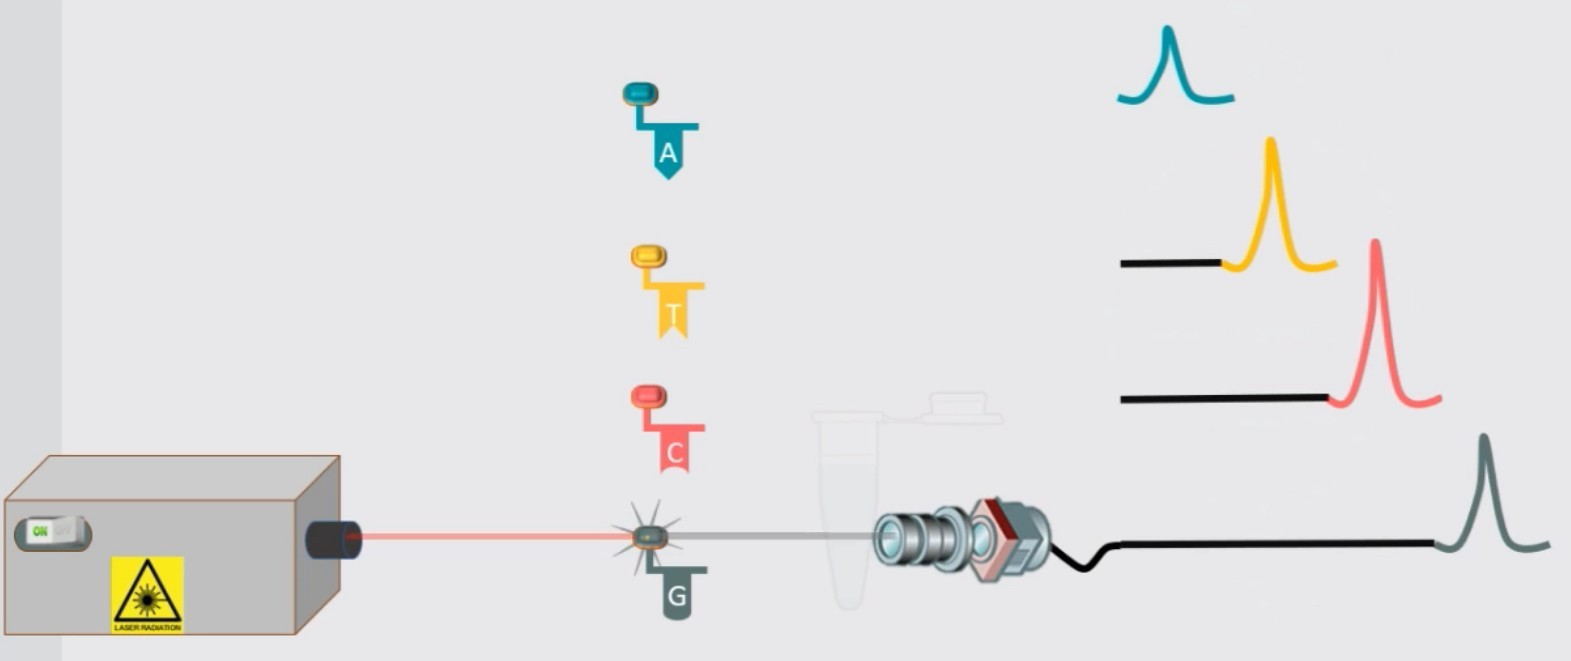
\includegraphics[width=\textwidth,height=0.7\textheight,keepaspectratio]{img/sequencing/seq30.jpg}
		\label{img:mot2}
		\caption{Each of the four ddNTPs chain terminator are labelled with fluorescent dyes.}
	\end{figure}
\end{frame}
%-------------------------------------------------------
%-------------------------------------------------------

%-------------------------------------------------------
%-------------------------------------------------------
\begin{frame}{Sanger method}{Capilar Electrophoresis}
	\begin{figure}[]
		\centering
		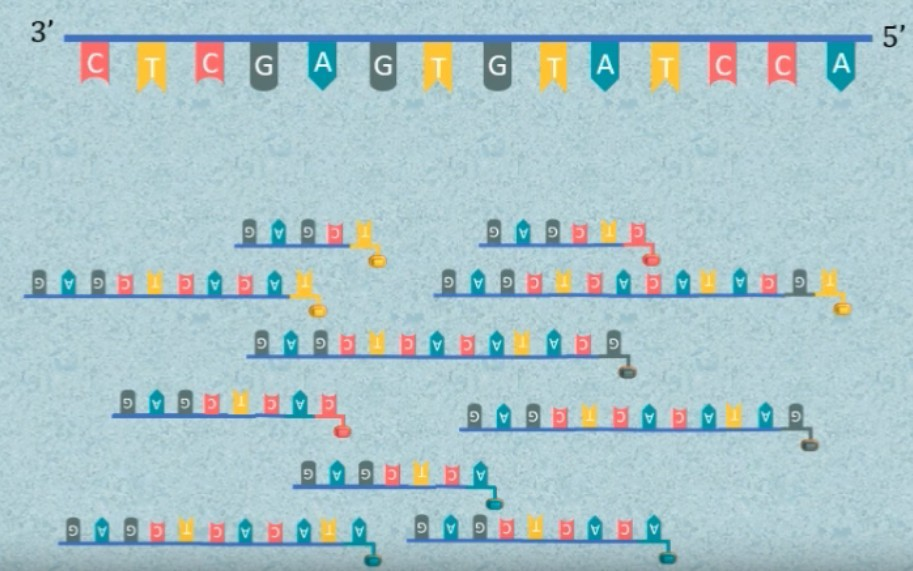
\includegraphics[width=\textwidth,height=0.7\textheight,keepaspectratio]{img/sequencing/seq31.jpg}
		\label{img:mot2}
		\caption{DNA replication occurs in one tube (Gel electrophoresis uses four).}
	\end{figure}
\end{frame}
%-------------------------------------------------------
%-------------------------------------------------------



%-------------------------------------------------------
%-------------------------------------------------------
\begin{frame}{Sanger method}{Capilar Electrophoresis}
	\begin{figure}[]
		\centering
		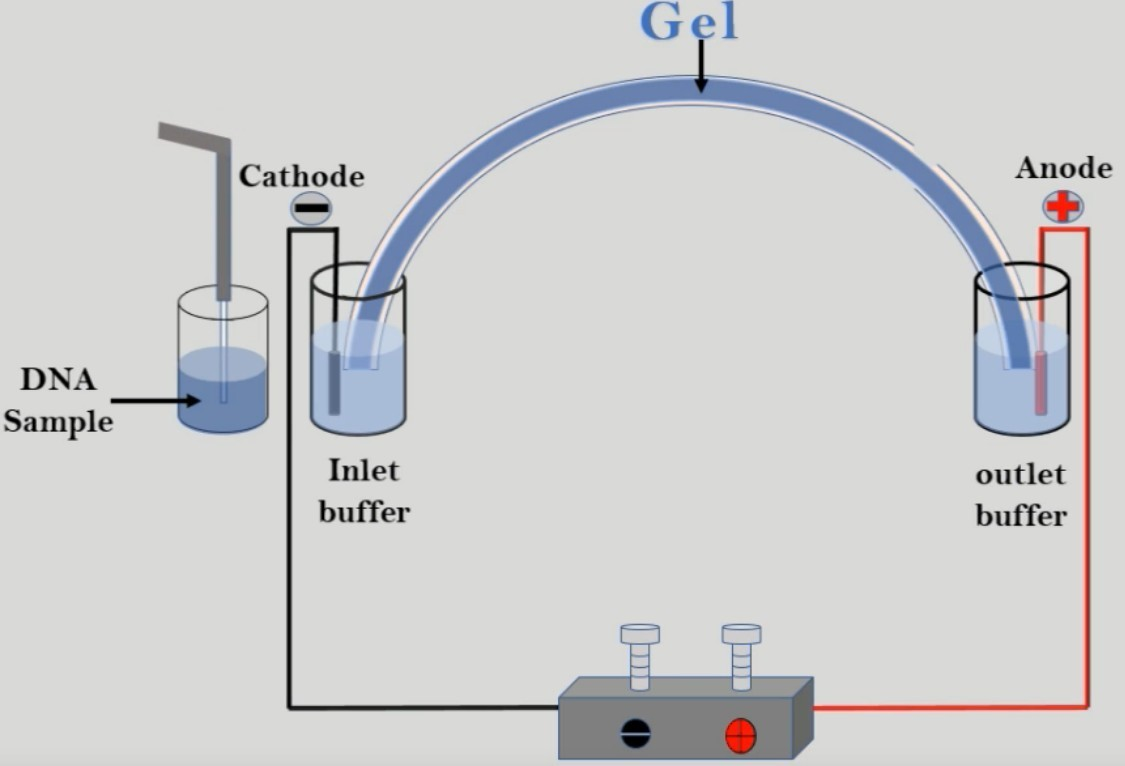
\includegraphics[width=\textwidth,height=0.7\textheight,keepaspectratio]{img/sequencing/seq32.jpg}
		\label{img:mot2}
		\caption{DNA fragments are placed in order move through a gel conductor.}
	\end{figure}
\end{frame}
%-------------------------------------------------------
%-------------------------------------------------------


%-------------------------------------------------------
%-------------------------------------------------------
\begin{frame}{Sanger method}{Capilar Electrophoresis}
	\begin{figure}[]
		\centering
		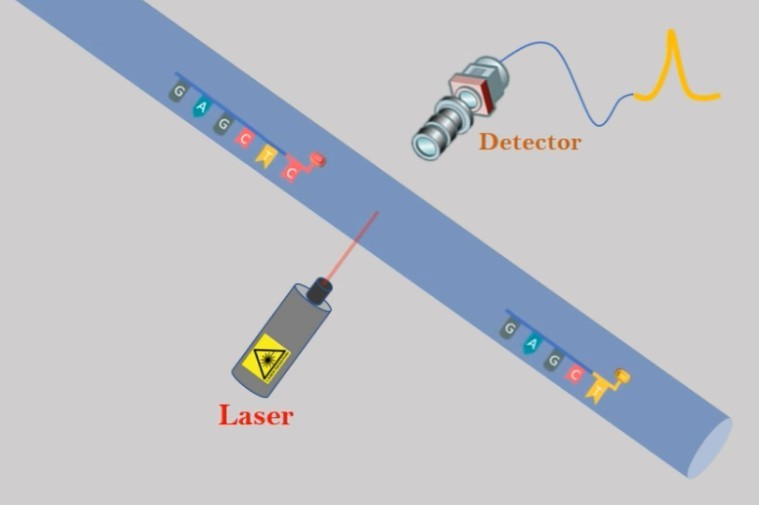
\includegraphics[width=\textwidth,height=0.5\textheight,keepaspectratio]{img/sequencing/seq20.jpg}
		\label{img:mot2}
		\caption{The fragment are charged and they move over a conductor. Smaller moves rapidly and they are read by a laser.}
	\end{figure}
\end{frame}
%-------------------------------------------------------
%-------------------------------------------------------

%-------------------------------------------------------
%-------------------------------------------------------
\begin{frame}{Sanger method}{Many samples read}
	\begin{figure}[]
		\centering
		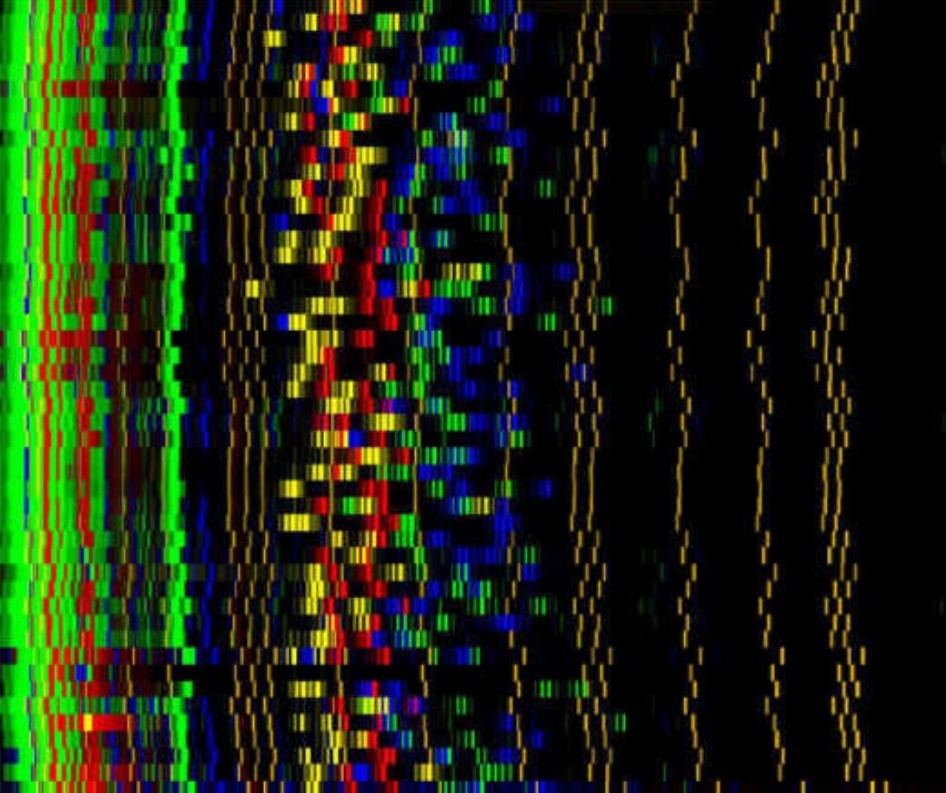
\includegraphics[width=\textwidth,height=0.5\textheight,keepaspectratio]{img/sequencing/seq22.jpg}
		\label{img:mot2}
		\caption{The process is repeated several times and many samples are obtained.}
	\end{figure}
\end{frame}
%-------------------------------------------------------
%-------------------------------------------------------



%-------------------------------------------------------
%-------------------------------------------------------
\begin{frame}{Sanger method}{Capillary Electrophoresis Animation}
	\begin{block}{}
		\href{https://www.youtube.com/watch?v=wdS3j0TgbjM&list=PLgM5s3vRHCgejiz7lKLR318mXs0ox4NFC&index=6&t=0s}{Capillary Electrophoresis Animation.}
		
	\end{block}
\end{frame}
%-------------------------------------------------------
%-------------------------------------------------------


%-------------------------------------------------------
%-------------------------------------------------------
\begin{frame}{Sanger method}{Gel Electrophoresis vs Capillary Electrophoresis}
	\begin{block}{}
		\begin{itemize}
			\item Capillary Electrophoresis is faster than Gel Electrophoresis.
			\item In Gel Electrophoresis the X-ray film is read by eyes meanwhile, in Capillary Electrophoresis a machine records the DNA sequence.
			\item Gel Electrophoresis reads DNA fragments of 150-200 bp meanwhile, Capillary Electrophoresis reads DNA fragments of 800-1000 bp.
		\end{itemize}
	\end{block}
\end{frame}
%-------------------------------------------------------
%-------------------------------------------------------

%-------------------------------------------------------
%-------------------------------------------------------
\begin{frame}[allowframebreaks]
        \frametitle{References}
        %\bibliographystyle{amsalpha}
        \bibliographystyle{IEEEtran}
        \bibliography{bibliography.bib}
\end{frame}
%-------------------------------------------------------
%-------------------------------------------------------

%-------------------------------------------------------
%-------------------------------------------------------
\if\mycmd1 % MY THEME
\1{
	{\1
		\begin{frame}[plain,noframenumbering]
			\finalpage{Thank you}
		\end{frame}}
		\else % CS THEME
		
\fi
%-------------------------------------------------------
%-------------------------------------------------------



\end{document}